% JuliaCon proceedings template
\documentclass{juliacon}
\usepackage{mathtools}
\usepackage{lipsum}

\setcounter{page}{1}

\nonstopmode

\begin{document}


% **************GENERATED FILE, DO NOT EDIT**************

\title{Julia Plasm Geometry for Solid Modeling}

\author[1]{Alberto Paoluzzi1}
\author[2]{Giorgio Scorzelli}
\affil[1]{Roma Tre University, Rome, Italy}
\affil[2]{Scientific Computing Institute, University of Utah, USA}

\keywords{Julia, Geometry, PLaSM, PyPlasm, Plasm.jl, BIM, CAD, DSL}

\hypersetup{
pdftitle = {Julia Plasm Geometry for Solid Modeling},
pdfsubject = {JuliaCon 2022 Proceedings},
pdfauthor = {Alberto Paoluzzi1, Giorgio Scorzelli},
pdfkeywords = {Julia, Geometry, PLaSM, PyPlasm, Plasm.jl, BIM, CAD, DSL},
}



\def\E{\mathbb{E}}
\def\R{\mathbb{R}}
\def\Z{\mathbb{Z}}
\def\N{\mathbb{N}}
\def\P{\mathbb{P}}
\def\v#1{{\bf #1}}
\def\p#1{{\bf #1}}
\def\T#1{{\bf #1}}

\maketitle


\begin{abstract}

In this presentation, we introduce the Julia implementation of the geometric functional language PLaSM (Programming Language for Solid Modeling), a geometry extension of the FL research language developed by Backus and his group at IBM Almaden. Implemented as a Julia package, Plasm.jl exploits the Julia programming environment to empower AEC (Architecture, Engineering, Construction) users and BIM (Building Information Modeling) developers with a robust DSL (Domain Specific Language) for architectural design and CAD. In this presentation, we synthesize the background, architecture, and data structures of Plasm.jl, which is well-founded on combinatorial topology, algebraic homology, and Boolean binary algebra. We also provide images and code demonstrating how simple the composition and application of geometric operators are to build solid objects and environments.

\end{abstract}



\tableofcontents

\section{Introduction}
\label{sec:additional_faci}

We present a synthesis of the Julia embodiment of the PLaSM programming DSL, a geometry-oriented, comprehensive collection of specialized operators and data types designed to assist AEC users and/or BIM programmers in generating complex parametric solid objects and assemblies. This is accomplished through the specialized tools offered by this Julia package for symbolic modeling. 

Cellular models, often called \emph{meshes} in engineering, design, and graphics, utilize \emph{discrete cells} to represent a geometric domain. In fields such as geospatial mapping, computer vision, robotics, graphics, finite element analysis, medical imaging, 3D printing, solid modeling, and geometric design, computing incidences, adjacencies, and mesh cell orderings typically depend on various incompatible data structures and algorithms. Plasm utilizes only Julia’s sparse matrices and vectors and a new homological method for building any Boolean expressions with union, intersection, and difference, and for visualization of models. 

This package also provides a general mechanism (Julia dictionaries) for exporting models characterized by colors, textures, materials, and more, including boolops among lower-level components. 

While Julia has many simple, efficient, and beautiful packages for elementary geometric shapes and constructions and visualization of numerical simulation results, it yet lacks general-purpose tools for building and discretizing complex and large-scale geometric assemblies. Also lacks Boolean solid operations, boundary evaluation and computation of surfaces, volumes, and inertia of models and/or their parts. Additionally, Plasm can be embedded in the Jupyter platform to document design choices within digital notebooks.

\subsection{FL origin of Plasm.jl package}
\label{sec:plasm}

In 1991, the Italian Research Council (CNR) financed a research program called “Edilizia” to promote and support national efforts to industrialize building construction. In this program, the Sapienza CADLab won a funding award sufficient to create and sustain a CS research group in geometric programming around the PLaSM project.
In the same year, on the track of Backus’ Turing Award, the functional programming group at IBM Almaden published the FL manual for function-level programming using combinatory logic. 

\subsection{First implementations}
\label{sec:pyplasm}
Developed under Italy's `Edilizia’ Finalized Project, Plasm may emerge as a pioneering metalanguage for Building Information Modeling (BIM). It evolved through multiple programming languages while retaining its core focus: multidimensional geometry and functional programming.

The PLaSM Group implemented the few combinators of FL \emph{algebra of programs} in Common Lisp, introducing a geometric type alongside the native ones: functions, numbers, characters, and sequences~\cite{BWW90,IBM:RJ7100}. The resulting DSL revealed an incredible descriptive power to generate multidimensional geometric models and assemblies in a few code lines~\cite{Paoluzzi2003a}. Years later, we opted for Scheme and a C\texttt{++} implementation of geometry kernel. After the move of A.P. to the new Roma Tre University and a SUR Award from IBM supporting all hardware and software (Catia licences) of a new PLM Laboratory, G.S. implemented the Pyplasm library, used to teach Computer Graphics and Geometric programming in Python and to model archeological sites like the emperor palaces on Palatine hill, S. Stefano Rotondo in Rome, and the leaning Pisa tower. Finally, while rethinking Booleans, we started porting the platform to Julia \cite{BEKS14}, where the geometry engine Plasm.jl and the book \cite{Plasm:book:2005} provide more recent and better results. 

\section{Solid representations and Julia data types}
\label{sec:additional_doc}

The foundations of solid modeling technology were established between the 70s and 80s. After 40 years, at Roma Tre we started exploring new paradigms~\cite{DBLP:journals/cad/DiCarloPS14,TSAS:2020,PAOLUZZI2023103436}, not based on computational geometry algorithms and data structures, but on novel abstractions taking into account structures and operators of algebraic topology and linear algebra, as is happening in modern AI.

A \emph{representation scheme} of solids is a mapping $r: M \to R$ between a space of mathematical models $M$ and a space of representations $R$ generated by a computer grammar.

\subsection{Plasm representation scheme}
\label{subsec:additional_doc}

Plasm.jl is a Julia package that maps any user-defined geometric expression to a binary expression of set algebras of geometric atoms, which may be resolved by linear operators on ALU engines. 

The mathematical domain of the representation scheme is the category of \emph{chain complexes}. The representation codomain space consists of \emph{Julia data types} where evaluated expressions are stored.

In simple terms, any \emph{model} is a chain (subset of cells in 0, 1, 2, or 3-dimensional linear chain space), and any \emph{representation} is an instance of Julia’s Hpc or Lar data types described below.

Our approach and Julia implementation originate from over fourteen years of research and experimental implementations focused on innovatively addressing the fundamental issue of solid modeling, i.e., Boolean operations. 


\subsection{Julia user-defined data types}
\label{subsec:title_auth}

Julia Plasm is based on three user-defined data types, enriched by several constructor and conversion methods:
\begin{description}
	\item[\textbf{Hpc}] \emph{Hierarchical Polyhedral Complex}, for hierarchical assembly, Boolean definitions, and interactive visualization on GPUs.
	\item[\textbf{Lar}] \emph{Linear Algebraic Representation}, for instancing and computing with boundary-based  cellular complexes and chain operators.
	\item[\textbf{Geo}] \emph{Geometry}, for enumeration of 0- $,\ldots,$ $d$-chains in hierarchical space domains, like octrees and potrees, and for $n$D partitions in convex or non-convex cells, together with Hpc or Lar objects.
\end{description}


\section{Geometric operators}
\label{sec:additional_faci}

In FL, the function-level approach focuses on composition, with new functions defined by combining existing tasks in various ways to create novel functions. This methodology yields a programming style centered on function-valued expressions. Few basic geometric operators in Plasm are defined without explicit arguments, departing from the applicative style. Most geometric operators utilize the functional style based on multiple applications supported by the Julia syntax, such as the $\circ$ composition operator.



\subsection{Affine Transformations}
\label{subsec:title_auth}

In geometric modeling and computer graphics, it is helpful to distinguish between a space of vectors and a space of points (supported by vectors). In Plasm, any geometric object (Hpc or Lar) is defined in a local Euclidean space. Any affine assembly or Boolean expression is described in the coordinate frame of its first object.  Internally, we use homogeneous normalized coordinates that are transparent to the users, with the homogeneous one in the first (no last) position.

\begin{figure}[h]
\centerline
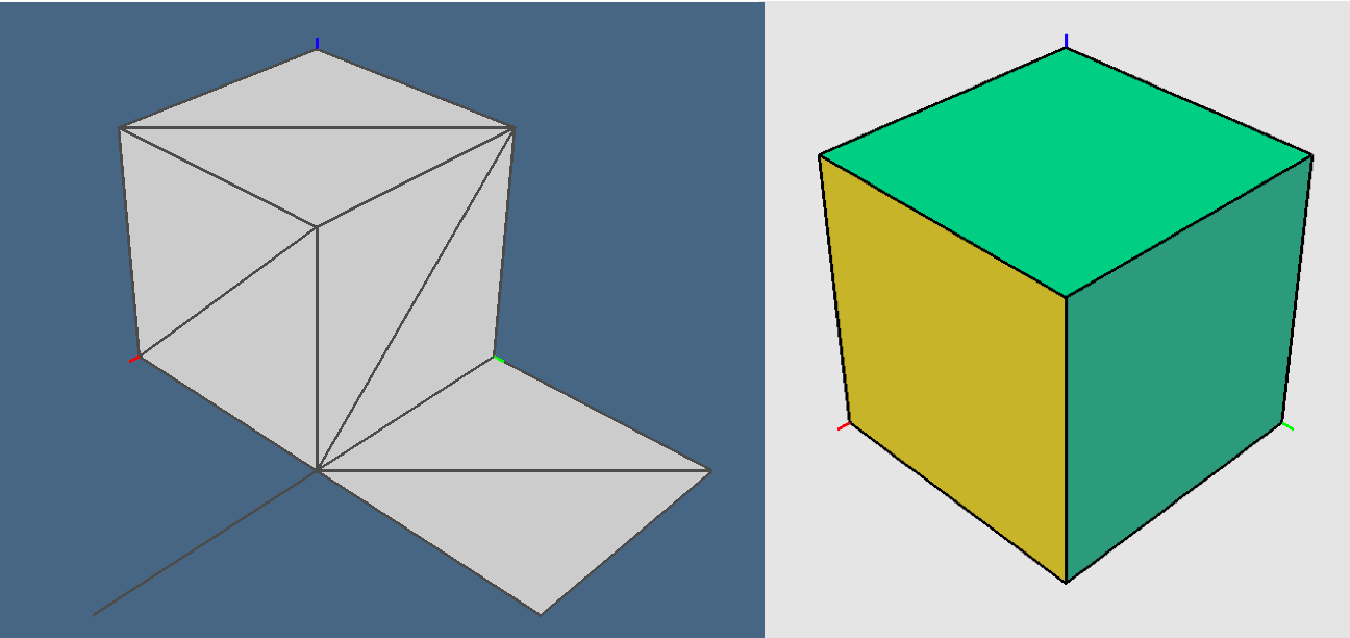
\includegraphics[width=\textwidth]{figs/cuboid}
\caption{Multidimensional {\tt hpc} assembly: (a) \texttt{STRUCT} object in default \texttt{VIEW}; (b) \texttt{VIEWCOMPLEX} of \texttt{LAR(hpc)} object.}
\label{sample-figure_2}
\end{figure}

In the following, we show three instances of application of \texttt{CUBOID},  and an assembly of \texttt{Hpc} type, shown on a white background, and assembled using the PHIGS+ semantics of \texttt{STRUCT}.
\begin{lstlisting}[
language = Julia,
numbers=none,
label={lst:exmpl1},
caption={Unit \texttt{interval} (1D), \texttt{square} (2D), \texttt{cube} (3D), and object \texttt{hpc} assembled with \texttt{STRUCT}.}
]
interval = CUBOID([1])
square = CUBOID([1,1])
cube = CUBOID([1,1,1])
hpc = STRUCT(cube,T(2)(1),square,T(1)(1),interval)
VIEW(hpc)
VIEWCOMPLEX(LAR(cube))
\end{lstlisting}

The \emph{affine transformation operators} require three applications to the coordinate indices, the transformation parameters, and an \texttt{Hpc} input object to generate a transformed \texttt{Hpc} output object. Two applications generate a geometry tensor as a partial function.  The number of indices is equal to the number of parameters and may range from 1 to $d$. All transformation tensors \texttt{T} (Translation), \texttt{R} (Rotation), \texttt{S} (Scaling), and \texttt{H} (Shearing) are multidimensional. All are implemented in Julia as partial functions using a square invertible matrix of normalized homogeneous coordinates, with the normalized one in the first position.


\subsubsection*{Translation transformation}\ 
\begin{lstlisting}[language = Julia,numbers=none,label={lst:exmpl2},
caption={Simple linear {\tt stair}, demonstrating an iterative use of tensors in {\small\tt STRUCT}. Of course, the number, size, and shape of the {\tt step} model can be parametrized as arguments of a geometric function returning {\tt Hpc} objects.}
]
function stairway(lx,ly,lz, n)::Hpc
	step   = QUOTE(lx) * QUOTE(ly) * QUOTE(lz)
	move   = T(1,2,3)(0, 0.8*ly, 0.8*lz)
	ramp   = STRUCT( CAT([[step, move] for k=1:n]) )
end 
stair = stairway(.8, .22, .18, 15);
VIEWCOMPLEX(LAR(stair))
\end{lstlisting}
\begin{figure}[htbp] %  figure placement: here, top, bottom, or page
    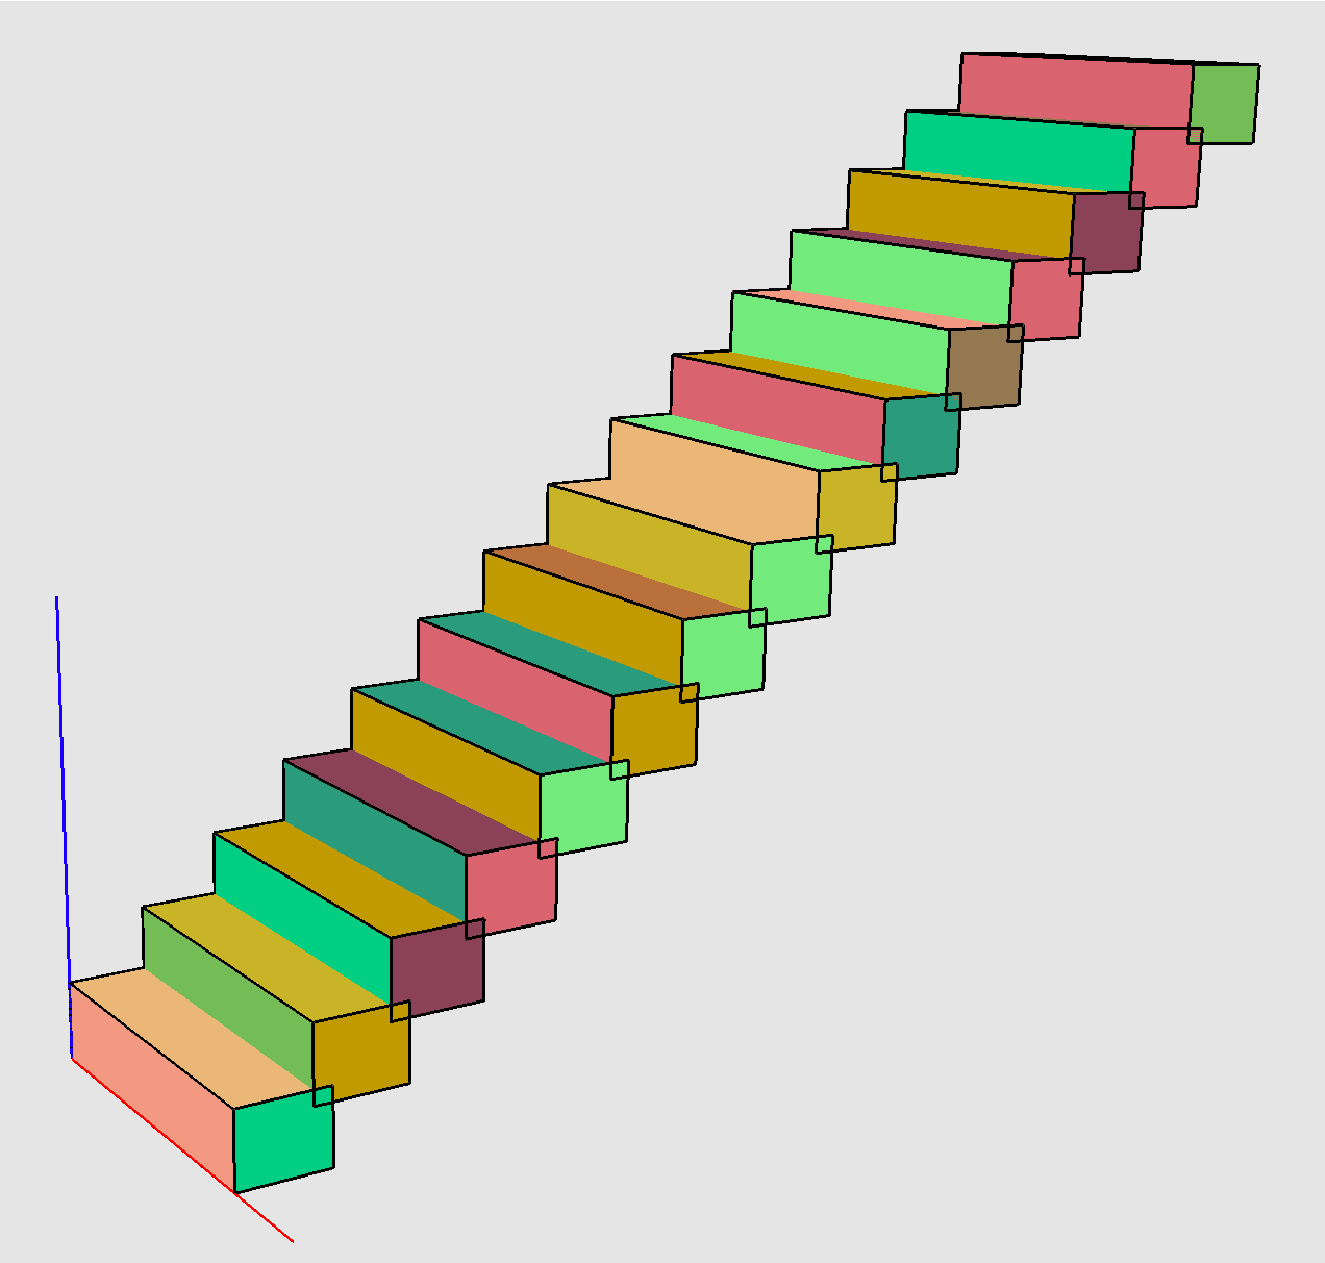
\includegraphics[width=0.35\linewidth]{figs/stair2}
     \caption{Number, size, and shape of the {\tt step} model can be parametrized as arguments of a function returning {\tt Hpc} objects.}
    \label{fig:stair}
\end{figure}


\subsubsection*{Rotation transformation}\ 
Two rotation parameters are used for elementary rotations in \emph{any} dimension, where only one coordinate is changed with the \texttt{sin} and \texttt{cos} pattern.

\begin{lstlisting}[language = Julia,numbers=none,label={lst:exmpl3},
caption={2D and 3D rotations.}
]
SQUARE(side) = CUBOID([side,side])		
obj = R(1,2)(π/4)(SQUARE(1)) # as 3D rot about z
VIEW(obj)

obj1 = R(2,3)(π/3)( CUBE(1) ); # rot about x 
obj2 = R(1,3)(π/6)( CUBE(1) ); # rot about y
obj3 = R(1,2)(π/4)( CUBE(1) ); # rot about z
VIEW( obj1 ); VIEW( obj2 ); VIEW( obj3 ); 
\end{lstlisting}
\begin{lstlisting}[
language = Julia,
numbers=none,
label={lst:exmpl4},
caption={Unit \texttt{interval} (1D), \texttt{square} (2D), \texttt{cube} (3D), and object \texttt{hpc} assembled with \texttt{STRUCT}.}
]
VIEWCOMPLEX(LAR(cube))
\end{lstlisting}
\begin{figure}[htbp] %  figure placement: here, top, bottom, or page
   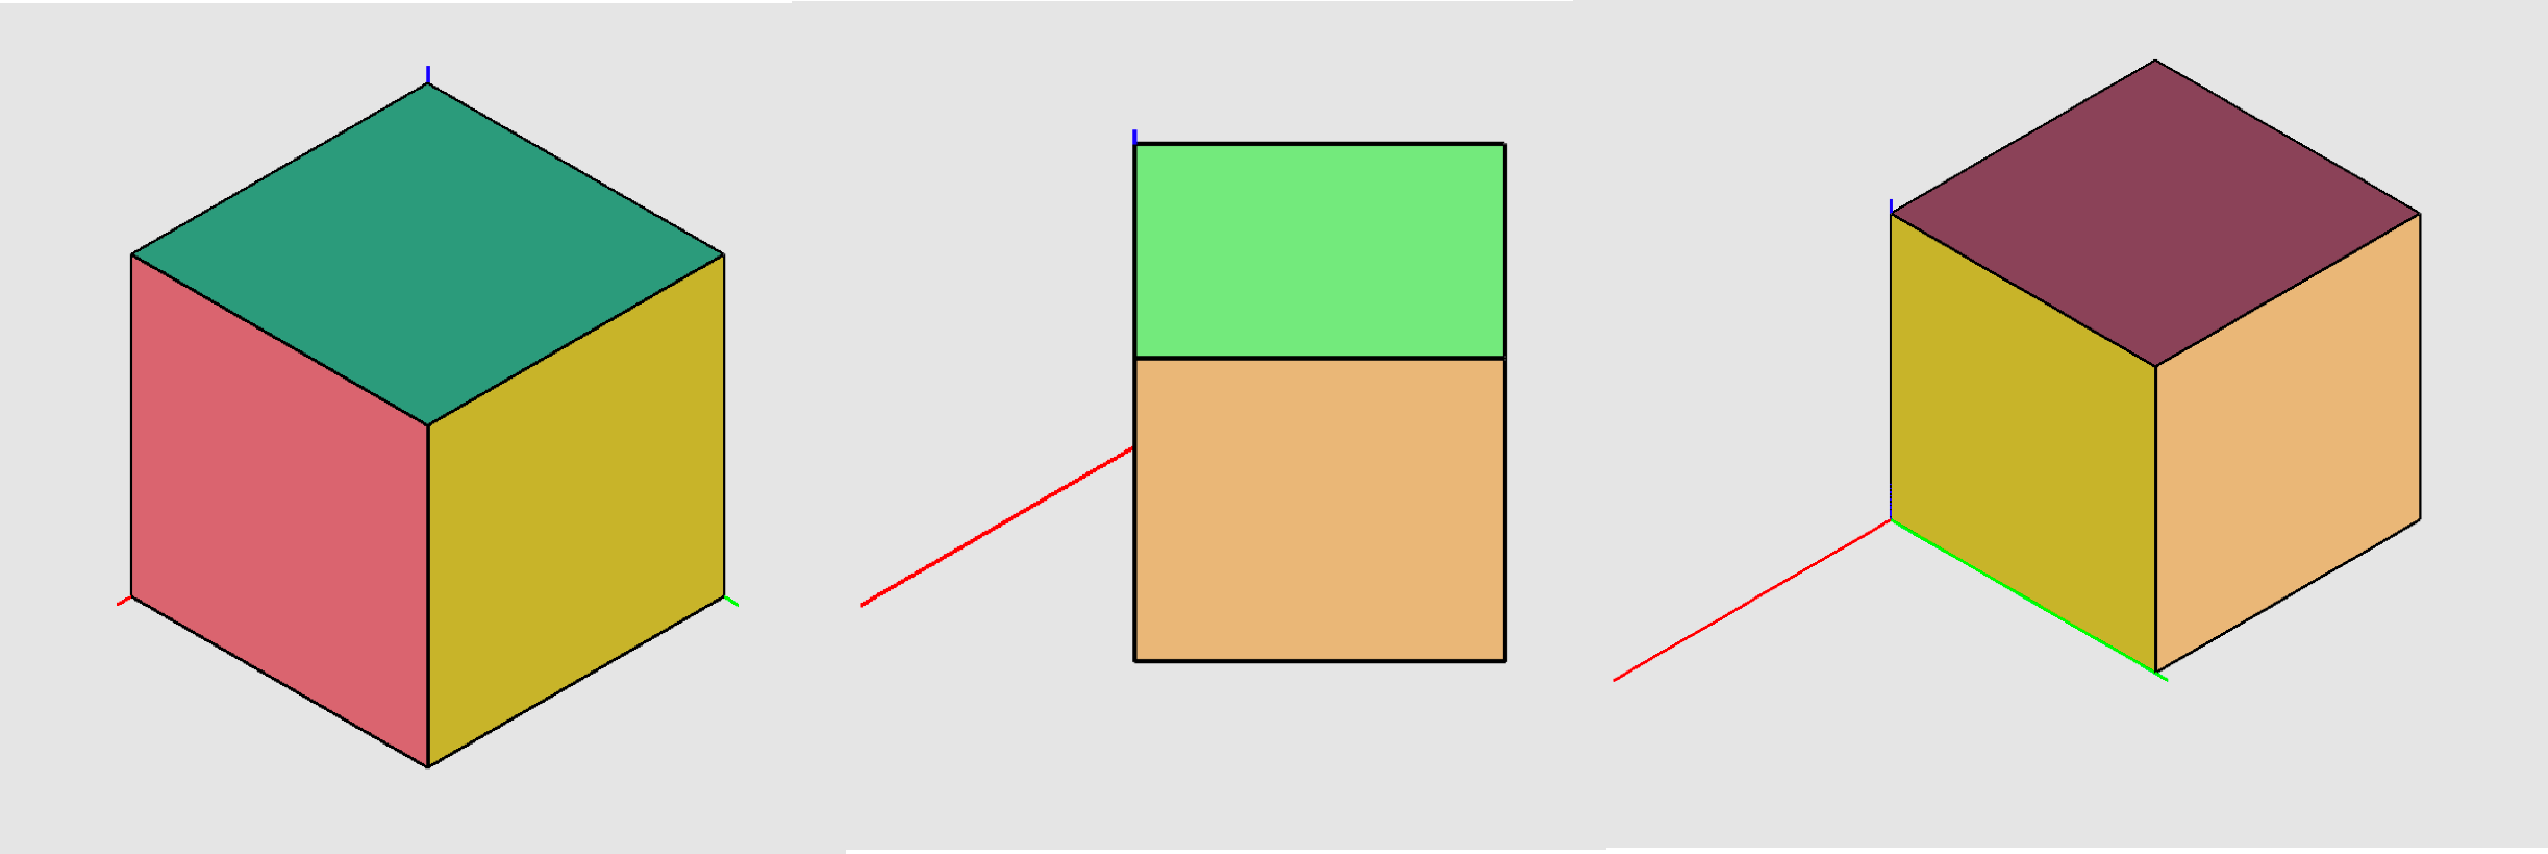
\includegraphics[width=\linewidth]{figs/3-cubes} 
   \caption{\scriptsize{Three parallel projections of a unit cube: {\tt
   V = VIEWCOMPLEX $\circ$ LAR; \\
   V(CUBE(1)); 
   V(R(1,2)($\pi$/4)(CUBE(1))); V(R(1,2)($\pi$/2)(CUBE(1))).}}}
   \label{fig:4:3-cubes}
\end{figure}


\subsubsection*{Scaling transformation}\ 
As an exciting coding example, we show how to construct an octahedron model simply by starting from the 3D SIMPLEX model. The final {\tt BOOL} operator produces a decompositive representation into four 3D tetrahedra (see Figure \ref{fig:octahedron}).

\begin{lstlisting}[language = Julia,numbers=none,label={lst:exmpl5},
caption={Construction of {\tt octahedron} model.}
]
tetra = HPCSIMPLEX(3);
twotetra = STRUCT( tetra, S(1)(-1), tetra );
fourtetra = STRUCT( twotetra, S(2)(-1), twotetra );
octahedron = BOOL(UNION( fourtetra, S(3)(-1), 
	fourtetra ))
VIEWCOMPLEX(octahedron,show=["CV"],explode=[2,2,2])
\end{lstlisting}
\begin{figure}[htbp] %  figure placement: here, top, bottom, or page
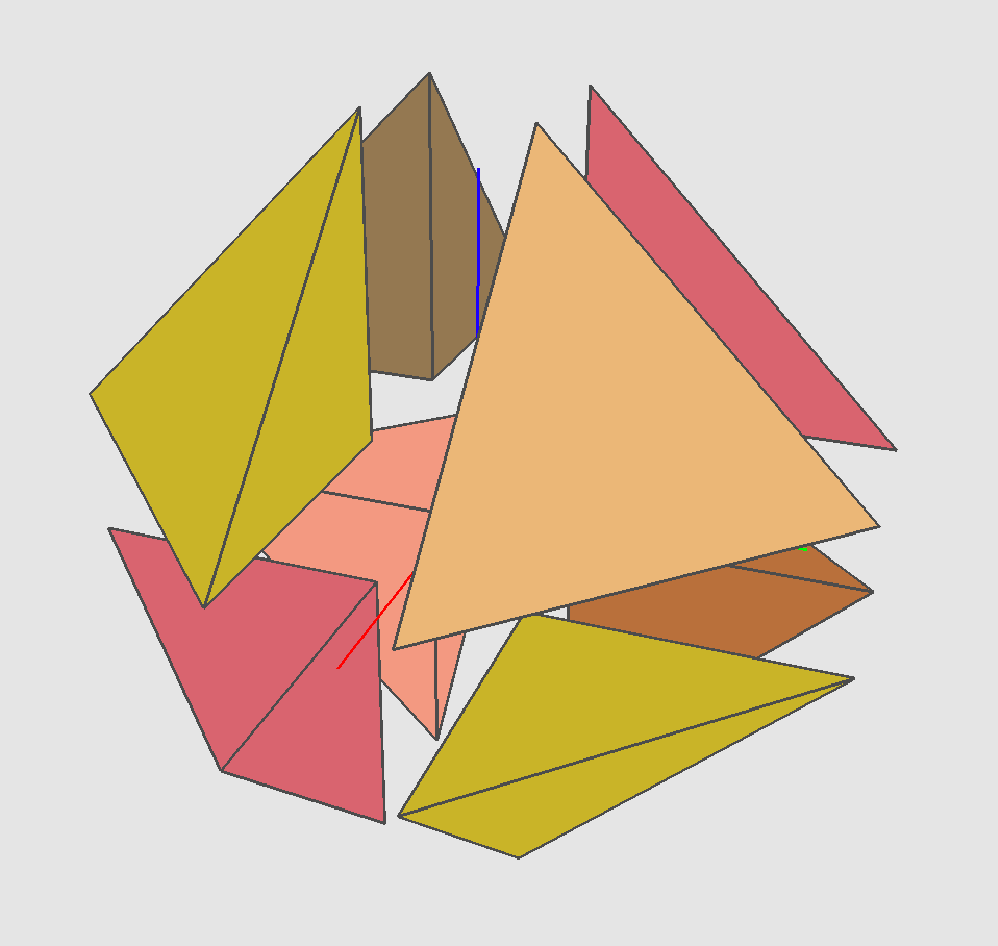
\includegraphics[width=0.5\linewidth]{figs/octahedron}
\caption{The {\tt octahedron} object’s atoms explosed. Notice that {\tt VIEWCOMPLEX} applies to {\tt Lar} values. The four atoms of the {\tt BOOL} operation are shown exploded (see \ref{sect:7:4:3} for details).}
\end{figure}
It is worth remarking that {\tt BOOL} is an alias for {\tt STRUCT}, where the \emph{boolops} associated with assembly subtrees are memorized inside the associated {\tt Hpc} subtrees {\tt Properties}.

\subsubsection*{Shearing transformation}\ 

\begin{lstlisting}[language = Julia,numbers=none,label={lst:exmpl6},
caption={3D shearing of the unit cube.}
]
shearedcube = H(3)(.2,.3)(CUBE(1))
VIEWCOMPLEX(LAR(shearedcube))
\end{lstlisting}
\begin{figure}[htbp] %  figure placement: here, top, bottom, or page
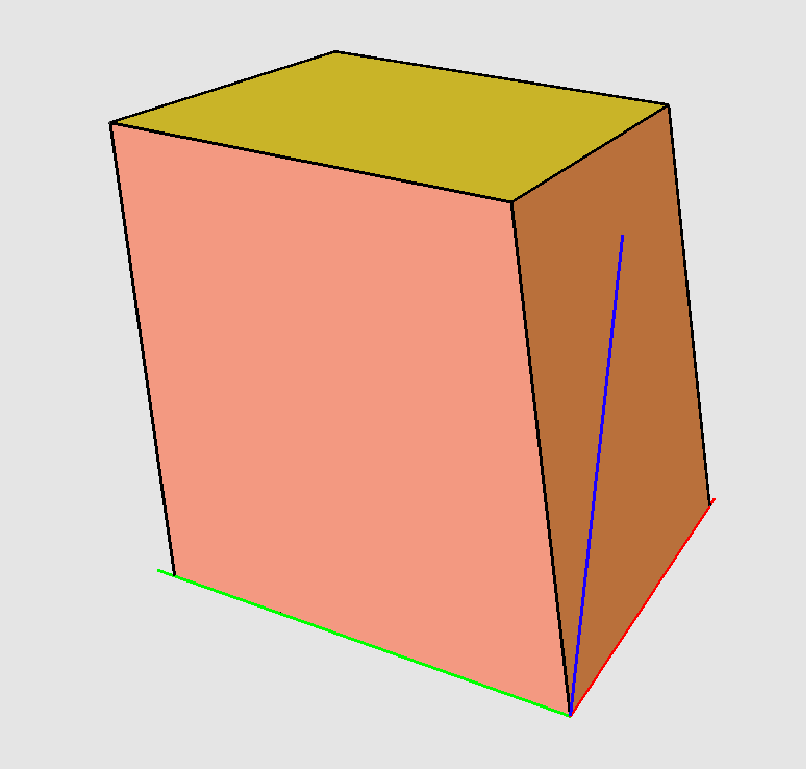
\includegraphics[width=0.5\linewidth]{figs/shearing3D}
\caption{Unit cube sheared on the (third) coordinate $z$. The $z$ of points does not change.}
\label{fig:4:shear:02}
\end{figure}
It is worthwhile to remark that the {\tt H} tensor, as {\tt R}, {\tt GR}, {\tt S}, 
{\tt T}, {\tt MAT}, and {\tt HOMO} are dimension independent, so they can be applied to models of whatever embedding dimension $d$ of geometric models. 
%Homogeneous \emph{normalized} matrices are used for implementation purposes. 


\subsection{Cellular and simplicial complexes}
\label{subsec:title_auth}

A cellular model, or mesh, represents a domain using discrete cells.

This section demonstrates that the Plasm representation scheme can be seen as a hybrid of cellular and boundary schemes \cite{Requicha:80}. Specifically, Plasm encapsulates a unique blend of hierarchical cellular schemas based on convex cell nodes defined by their vertices, alongside a flat scheme representing the entire topology of such assemblies. Importantly, chain complex representations avoid the issues and complications associated with geometric non-manifoldness, which need not be considered.

\subsubsection*{Cartesian product of complexes}

Let us introduce the definition of the multidimensional \emph{grids} of \emph{cuboidal}, and the general \emph{Cartesian product} {\tt *} of cellular complexes, also referred to as \emph{topological product}, which is commutative and associative like the standard product of numbers.
The {\tt *} operator, depending on the input’s dimension, generates either \emph{full-dimensional} output complexes or \emph{lower-dimensional} complexes of dimension $d$ embedded in Euclidean $n$-space, with $d \leq n$. We say an object is \textit{solid} when $d = n$.


\begin{lstlisting}[language = Julia,numbers=none,label={lst:exmpl7},
caption={Cartesian Product of 0/1 chain instances.}
]
grid1D = QUOTE(N(10)(.1));
grid2D = grid1D * grid1D;
grid3D = grid2D * grid1D;
grid11d = SKELETON(1)(grid2D);
VIEW(grid11d); VIEW(grid2D); VIEW(grid3D)
\end{lstlisting}
{\tt N(10)(.1)} creates an array of {\tt 10} values {\tt 0.1}. The operator {\tt QUOTE} transforms it into a 1D complex, i.e., a sequence of line segments. Figure \ref{ex:build1D} shows pictures of a 2D and 3D cuboidal complex.
\begin{figure}[h]
	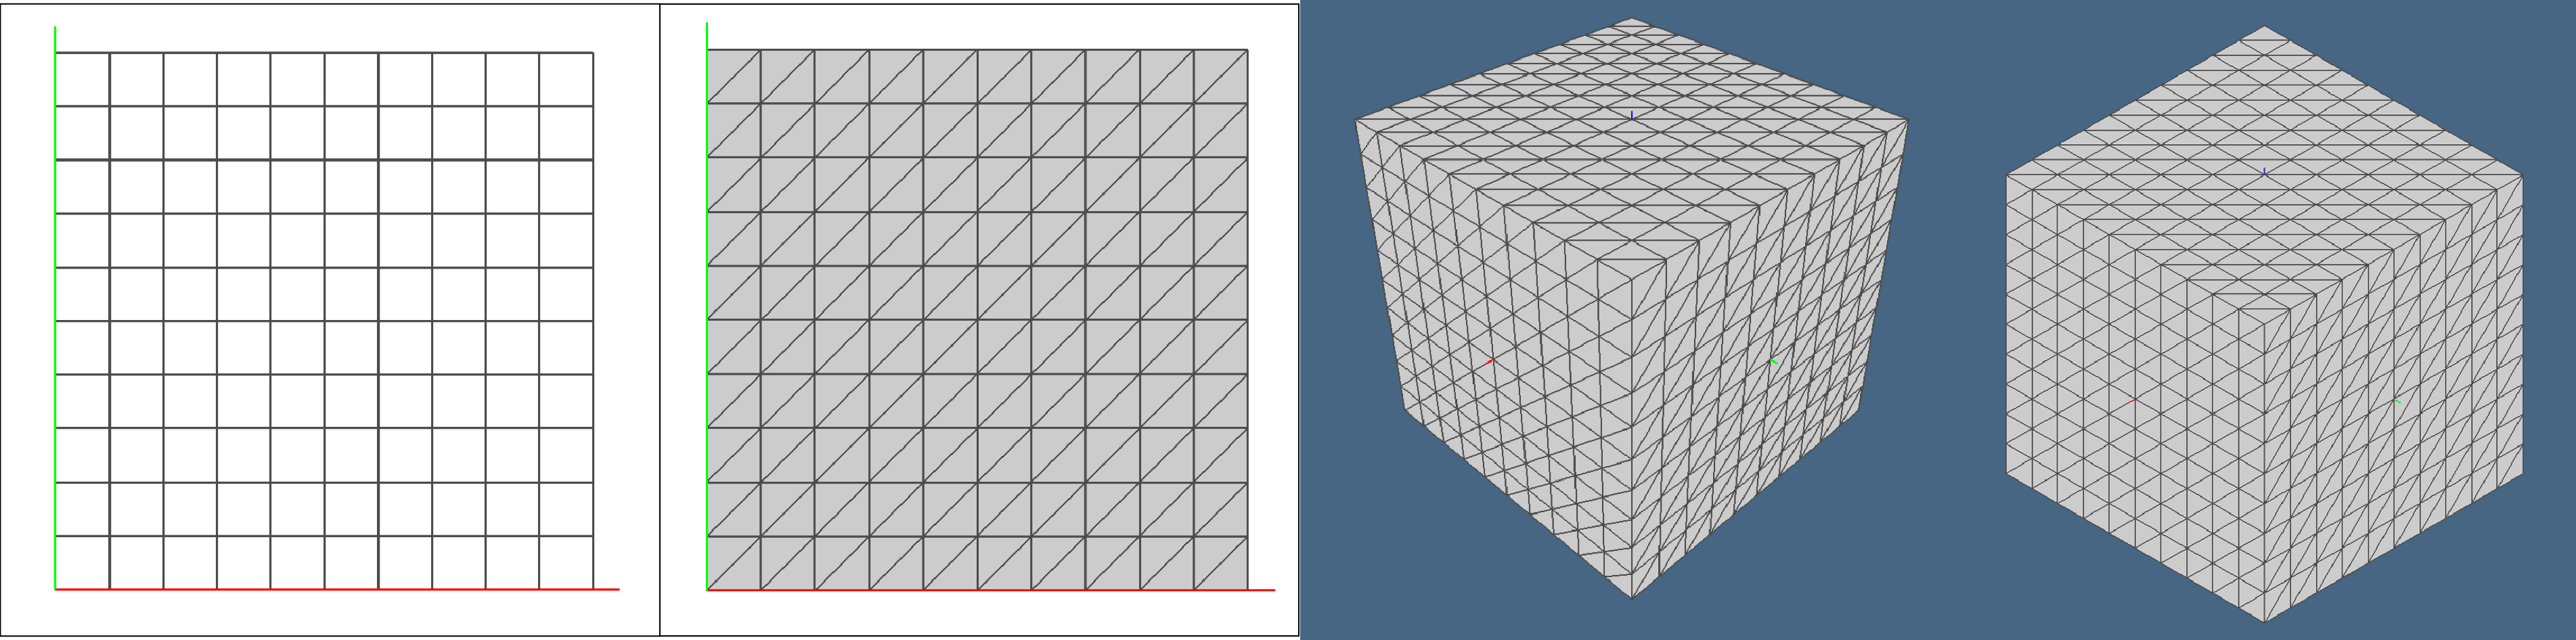
\includegraphics[width=\linewidth]{figs/four-grids}%
	\caption{Cellular complex: (a) 1-complex; (b) 2-complex; (c) 3-complex with perspective projection; (d) 3-complex with isometric parallel projection.}    \label{ex:build1D}
\end{figure}



We recall that a convex 3D cell may be represented (a) as the convex hull of its vertices (in Julia Plasm by the {\tt Hpc} data type), or by its Brep, boundary representation used locally or globally:
\begin{lstlisting}[language = Julia,numbers=none,label={lst:exmpl8},
caption={Direct gereration of any-dimensional cuboidal complex.}
]
 grid = CUBOIDGRID([2,3,1]) # Lar
 VIEWCOMPLEX(grid,explode=[1.2,1.2,2])
 
 julia> grid.C
Dict{Symbol, Vector{Vector{Int64}}} with 5 entries:
  :CF => [[1, 2, 4, 9, 11, 13], [2, 3, 7, 10, 15,...
  :CV => [[1, 2, 3, 4, 5, 6, 7, 8], [1, 2, 7, 8, ...
  :FV => [[1, 2, 3, 4], [1, 2, 7, 8], [1, 2, 13, ...
  :EV => [[1, 2], [1, 3], [1, 7], [1, 9], [1, 13],..
  :FE => [[1, 2, 6, 9], [1, 3, 7, 17], [1, 5, 8, ...
\end{lstlisting}
	\begin{figure}[htbp]  \centering
		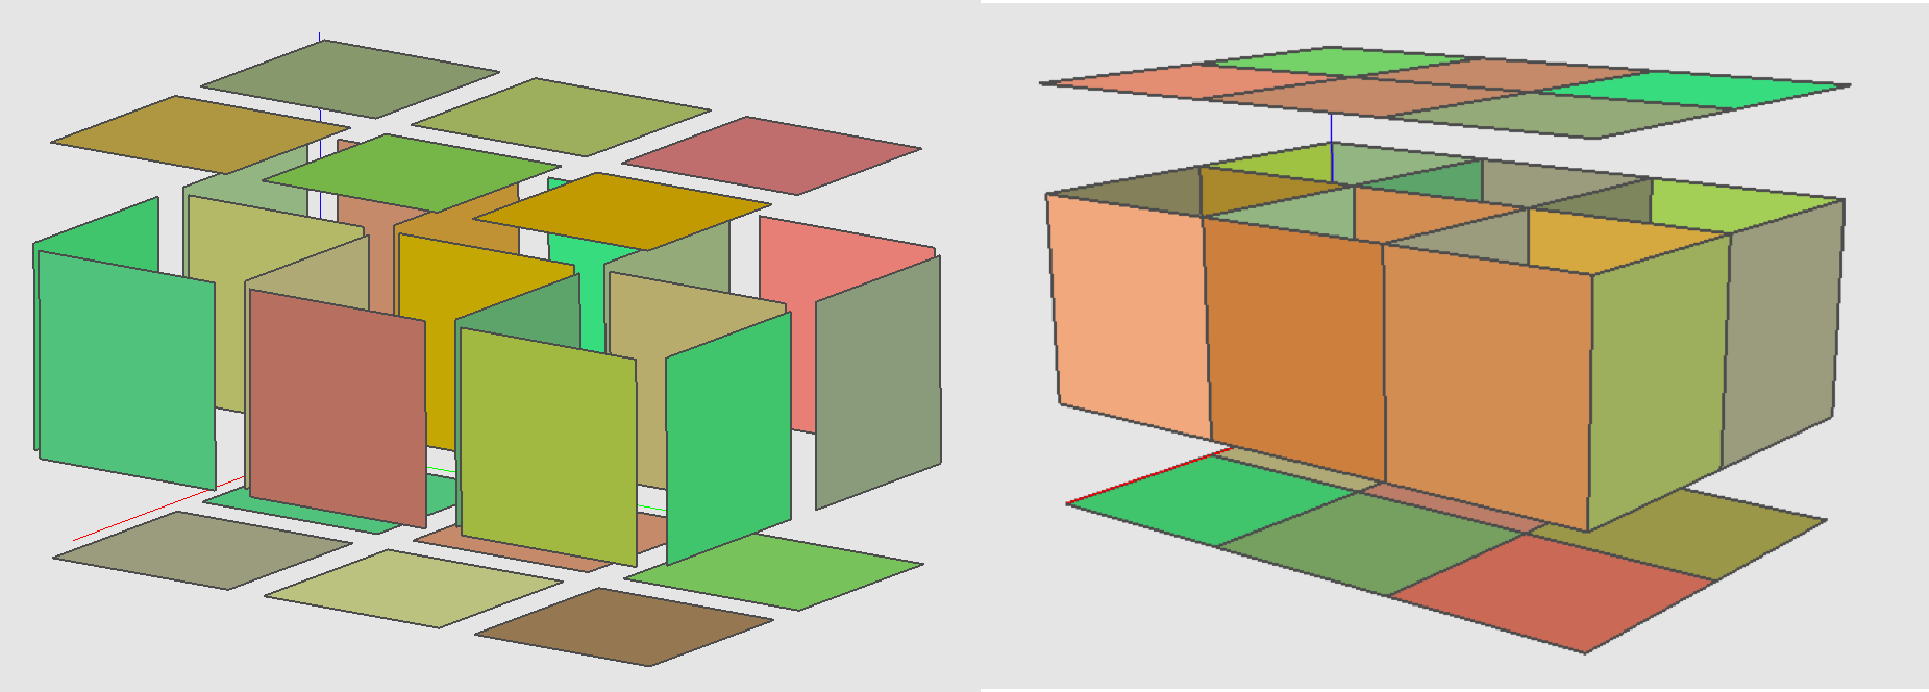
\includegraphics[width=0.75\linewidth]{figs/grid}
		\caption{Non-manifold internal brep, important with new materials models.}
		\label{grid}
	\end{figure}
	A small 3D {\tt grid} is exploded in Figure \ref{grid}. The complexes generated by {\tt CUBOIDGRID} are strongly non-manifold, an essential issue in designing a \emph{new representation} for solid modeling.
	The \texttt{Plasm} DSL and its Julia structures make the distinction between manifold and non-manifold objects and models obsolete. Using chain complex models, \emph{manifoldness} and its reverse property are not needed.


\subsubsection*{Simplicial extrusion of complexes}\label{rem:sixtetra}
The unit cube can be decomposed into six well-assembled unit tetrahedra (3-simplices), looking at Figure \ref{fig:tetgen2}, where a standard 2-simplex in $\E^2$ is extruded orthogonally in $\E^3$ to generate three standard 3-simplices, thus producing a half-cube partition. 
	

\begin{figure}[htbp] %  figure placement: here, top, bottom, or page
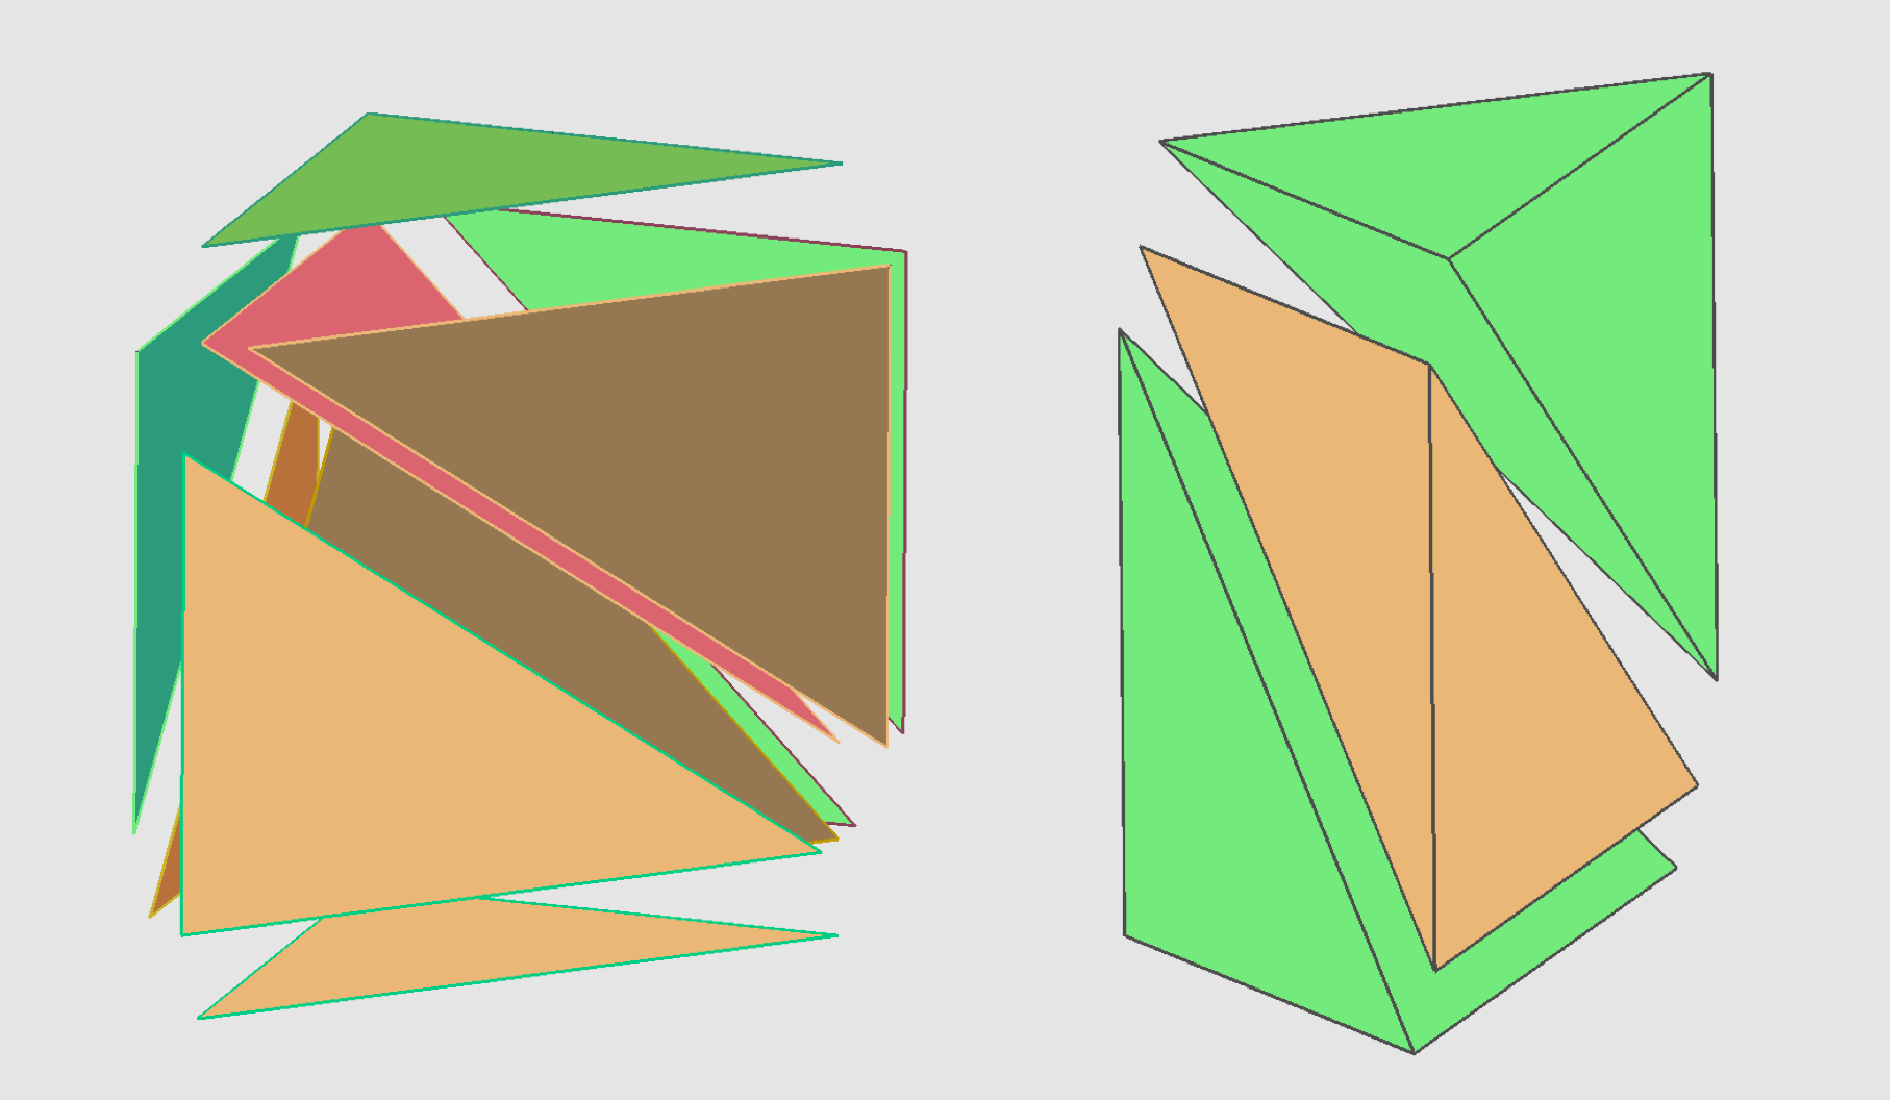
\includegraphics[width=0.5\linewidth]{figs/simplex-extrude}%
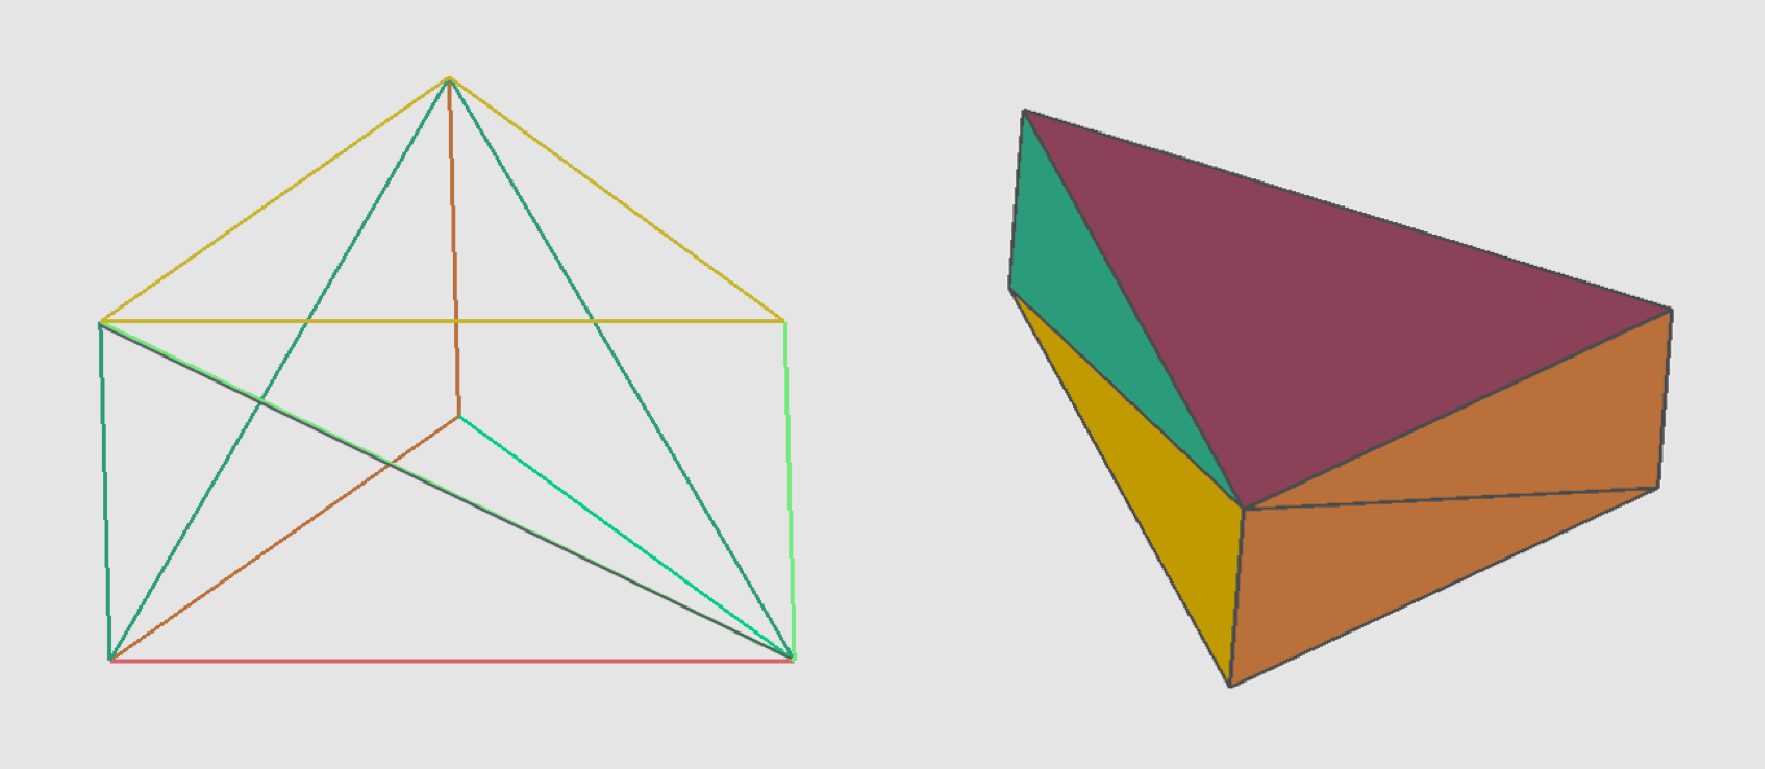
\includegraphics[width=0.5\linewidth,height=0.293\linewidth]{figs/half-cube-sk}
		\caption{Simplicial complex extrusion of the 2D triangle in $\E^2$, producing the half-cube in $\E^2$ as a complex with three tetrahedra: (a) 2-skeleton of exploded half-cube; (b) exploded 3-cells (tetrahedra);
(c) 1-skeleton (set of 1-cells); (b) 2-skeleton (set of 3-cells).}
\label{fig:tetgen2}
\end{figure}

A classic {\tt PLaSM} object {\tt model} is a {\tt Pair} (vertices, cells) to be extruded, whereas {\tt pattern} is an array of numbers for lateral measures of the \textbf{extruded model}, which enjoys one added dimension. The pattern’s elements are assumed as either \emph{solid} or \emph{empty} measures, according to their (+/-) sign.


\begin{lstlisting}[language = Julia,numbers=none,label={lst:exmpl9},
caption={Multiple Hpc model extrusion.}
]
V = [[0.,0] [1,0] [2,0] [0,1] [1,1] [2,1] [0,2] [1,2] [2,2]];
FV = [[1,2,4],[2,3,5],[3,5,6],[4,5,7],[5,7,8],[6,8,9]];
pattern = repeat([1,.2,-2],outer=4);
model = (V,FV)
W,FW = EXTRUDESIMPLICES(model, pattern);
VIEW(MKPOL(W,FW))
VIEWCOMPLEX(LAR(MKPOL(W,FW)))
\end{lstlisting}


\begin{figure}[htbp] %  figure placement: here, top, bottom, or page
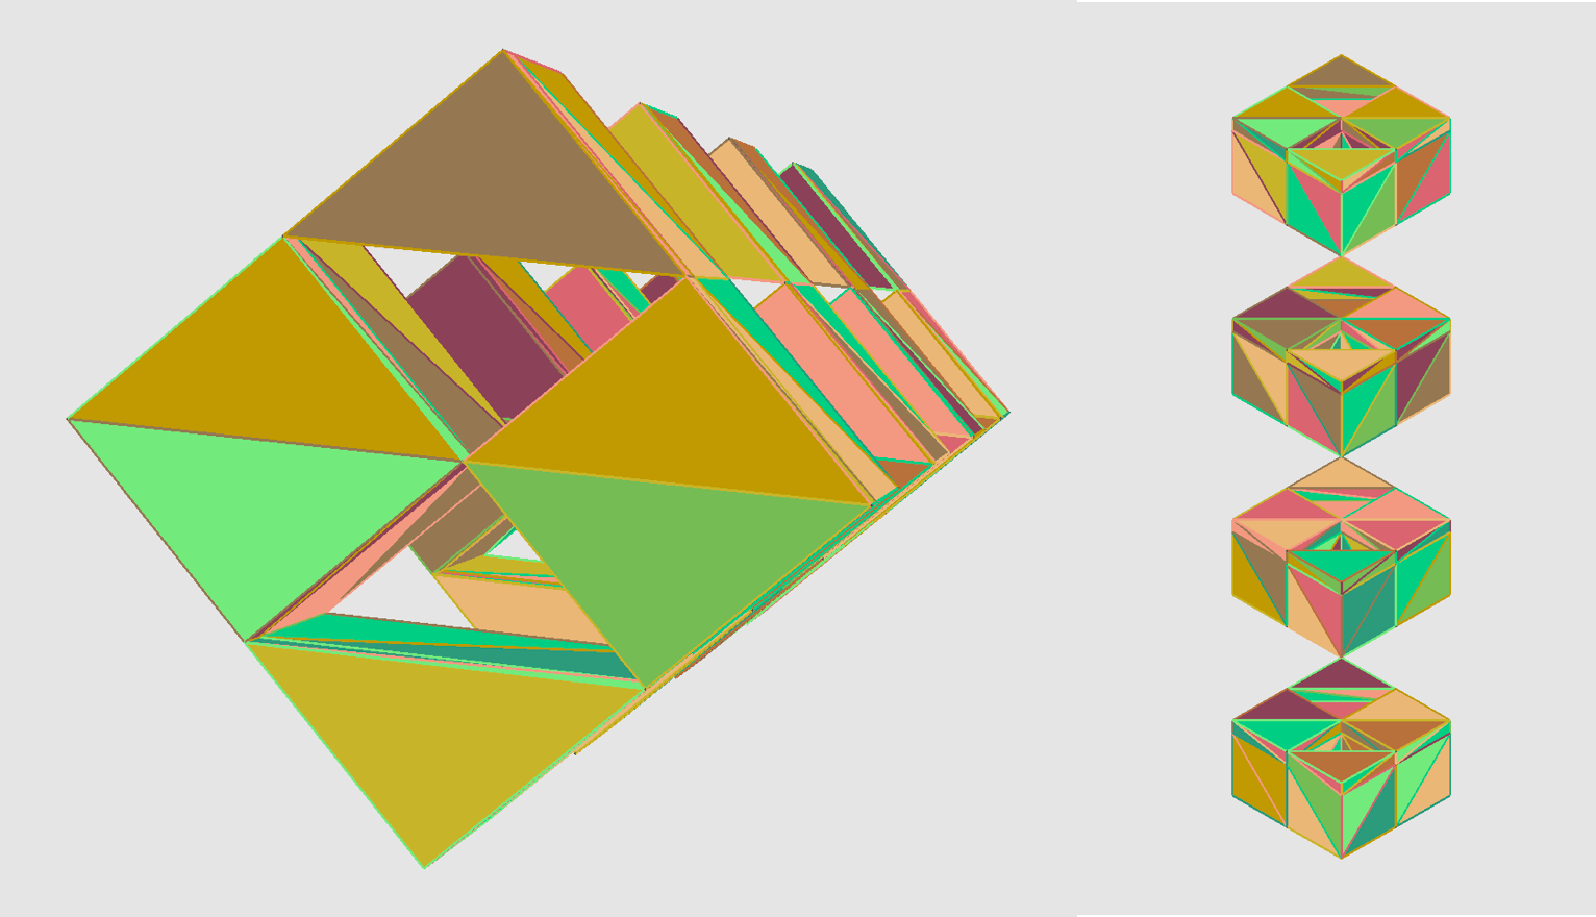
\includegraphics[width=\linewidth]{figs/multi-extrusion-02}
\caption{A highly no-manifold {\tt Plasm} model: (a) projective view of extruded 3-complex; (b) parallel view of 3-complex in $\E^3$.}
\label{fig:multi-extrusion-02}
\end{figure}


\subsubsection*{Simplicial grids}\ 


Geometric grid structure made by simplicial cells of the same dimension aligned on a cuboidal layout grid of 1D, 2D, 3D, etc., elements. For this construction, we use a multidimensional combinatorial formula to produce the output complex in $\Omega(n)$, linear with the output size.

This operator is mainly used for regular \emph{domain decomposition}, to {\tt MAP} any $d$ coordinate functions to create curved structures, such as proper curves, curved surfaces, and curved solids.
The curved complex is easily generated by applying the {\tt MAP} operator of Julia Plasm to some {\tt Hpc} grid, so that all vertex points are coherently transformed without changing the grid topology.

\begin{lstlisting}[language = Julia,numbers=none,label={lst:exmpl10},
caption={Multidimensional grid generation.}
]
grid = MKPOL(SIMPLEXGRID([10,10,1]))::Hpc
VIEWCOMPLEX(LAR(SKELETON(1)(grid))::Lar)
\end{lstlisting}

\begin{figure}[htbp] %  figure placement: here, top, bottom, or page
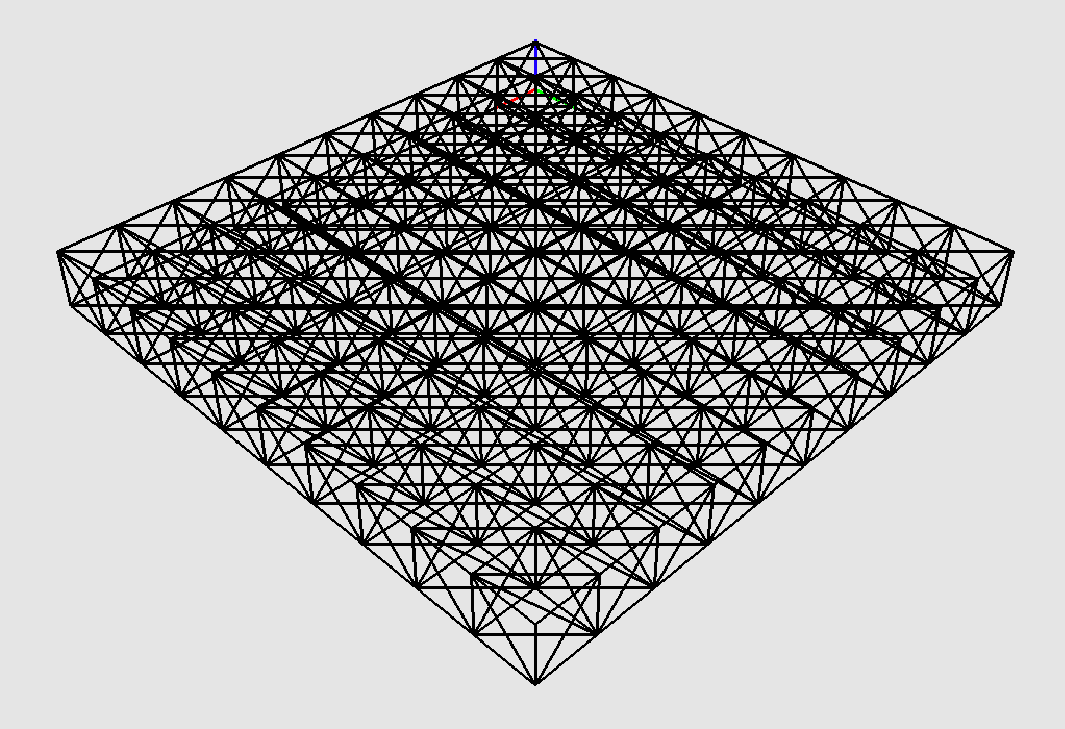
\includegraphics[width=\linewidth]{figs/3Dgrid}
\caption{ The {\tt SKELETON} operator extracting here the 1-complex from the well-assembled  3-complex generated by the {\tt SIMPLEXGRID} operator.}
\label{fig:multi-extrusion-02}
\end{figure}
The above is a slab scaffolding well-known to engineers. 
Because the structure is based on a triangulated framework (with triangles being inherently stable and resistant to deformation), and because these rigid cells are assembled in a regular grid, the load is efficiently distributed throughout the entire assembly. 

\subsubsection*{Volume integration of polynomials}
{Plasm.jl} also includes functions for calculating {domain integrals} of polynomials on piecewise-linear polyhedra \cite{CATTANI1990130} from a triangulation of the boundary of the domain model, an important solid modeling tool. In particular, Plasm has simple primitives for determining the mechanical properties of solids, including area, volume, centroid, products, and moments of inertia of models, presented in both scalar and tensor forms. 

Hopefully, readers will appreciate the remarkable compactness of the classic FL-based language PLaSM ported to Julia. 


\begin{lstlisting}[language = Julia,numbers=none,label={lst:exmpl10, mathescape = true},
caption={Boundary triangulation primitives.}
]
BREP(obj::Hpc) = CONS([S1,CAT \circ S2])(
	get_oriented_triangles(obj))
BREP(obj::Lar) = CONS([S1,CAT \circ S2])(
	get_oriented_triangles(MKPOL(obj.V,
		obj.C[:CV])))
\end{lstlisting}
Here, we have shown a compact API and FL-based implementation for a minimal  {\tt Plasm} interface that converts {\tt Hpc} and {\tt Lar} data objects into the model data structure recognized by the native {\tt PlaSM} language. 


The simplest test examples are given below, as usual when writing unit tests for software development.
Now compute some integrals on {\tt Hpc} dataset:
\begin{lstlisting}[language = Julia,numbers=none,label={lst:exmpl10},
caption={Simple test examples of the integration module {\tt Plasm/src/integr/}: volume, surface, and centroid tests.}
]
obj = CUBE(2) # => 3D cube of side 2
VOLUME(BREP(obj::Hpc)) # => 8
SURFACE(BREP(obj::Hpc)) # => 24
CENTROID(BREP(obj))' 
1x3 adjoint(::Vector{Float64}) with eltype Float64:
 1.0  1.0  1.0
\end{lstlisting}
Note that the operator {\tt BREP} only works with {\tt Hpc} objects. A {\tt Lar} object must first be transformed into the {\tt Hpc} data type. 




\subsection{Parametric curves, surfaces, and solids}
\label{subsec:title_auth}

This section is based on concepts essential for understanding computer-generated parametric
curves and surfaces. Specifically, we introduce the concepts of \emph{curve} and \emph{surface} as point-valued functions of one or two variables, respectively. 

Plasm restricts its curved geometric objects to manifold ones, where the neighborhood of any point is topologically equivalent to a small circle of the same dimension. This suffices to define limited regular surface \emph{patches}, the familiar curved objects in CAD and BIM. Each Plasm patch of a $d$-manifold is generated by mapping a vector function of $d$ coordinate functions over a cellular decomposition of the patch domain. To generate a 2D surface, i.e., a two-dimensional manifold embedded in $\E^3$, we need a vector-valued function with three coordinate functions of two parameters: $S(u,v) = [x(u,v), y(u,v), z(u,v)]$.
Some examples follow.

\begin{lstlisting}[language = Julia,numbers=none,label={lst:exmpl10},
caption={Symbolic example of Plasm-generated manifold patch. Of course, this coding structure may be modified when useful to produce a simpler user interface.}
]
patch = MAP(mapping)(domain)
\end{lstlisting}

\vspace{-5mm}
\begin{lstlisting}[language = Julia,numbers=none,label={lst:exmpl10},
caption={Transfinite Bézier patch defined by four Bézier curves. The corresponding surface patch is shown in Figure \ref{}. Note that the argument Bézier functions may have any degree.}
]
C0 = BEZIER(S1)([[0,0,0],[10,0,0]])
C1 = BEZIER(S1)([[0,2,0],[8,3,0],[9,2,0]])
C2 = BEZIER(S1)([[0,4,1],[7,5,-1],[8,5,1],[12,4,0]])
C3 = BEZIER(S1)([[0,6,0],[9,6,3],[10,6,-1]])
VIEW(MAP(BEZIER(S2)([C0,C1,C2,C3]))(
 	INTERVALS(1.0)(10) * INTERVALS(1.0)(10)))
\end{lstlisting}


\vspace{-5mm}
\begin{lstlisting}[language = Julia,numbers=none,label={lst:exmpl10},
caption={Specialized transfinite {\tt Bézier mapping}. Five control points, hence a quartic Bezier curve. Unit interval domain.}
]
controlpoints = [[0,0],[1,0],[0.5,2],[2,1],[2,2]]
curve  = BEZIER(S1)(controlpoints)
domain = INTERVALS(1.0)(32)
VIEW(STRUCT(
	COLOR(CYAN)(MAP(curve)(domain)), 
	COLOR(YELLOW)(POLYLINE(controlpoints)), FRAME2)) 
\end{lstlisting}

Many more curves, surfaces, and splines, including non-uniform B-splines and non-uniform rational B-splines (NURBs), have been ported to Plasm.jl from the classic PLaSM \cite{Paoluzzi2003a}. Two simple examples are given here. 

\begin{figure}[htbp] %  figure placement: here, top, bottom, or page
   \centering
   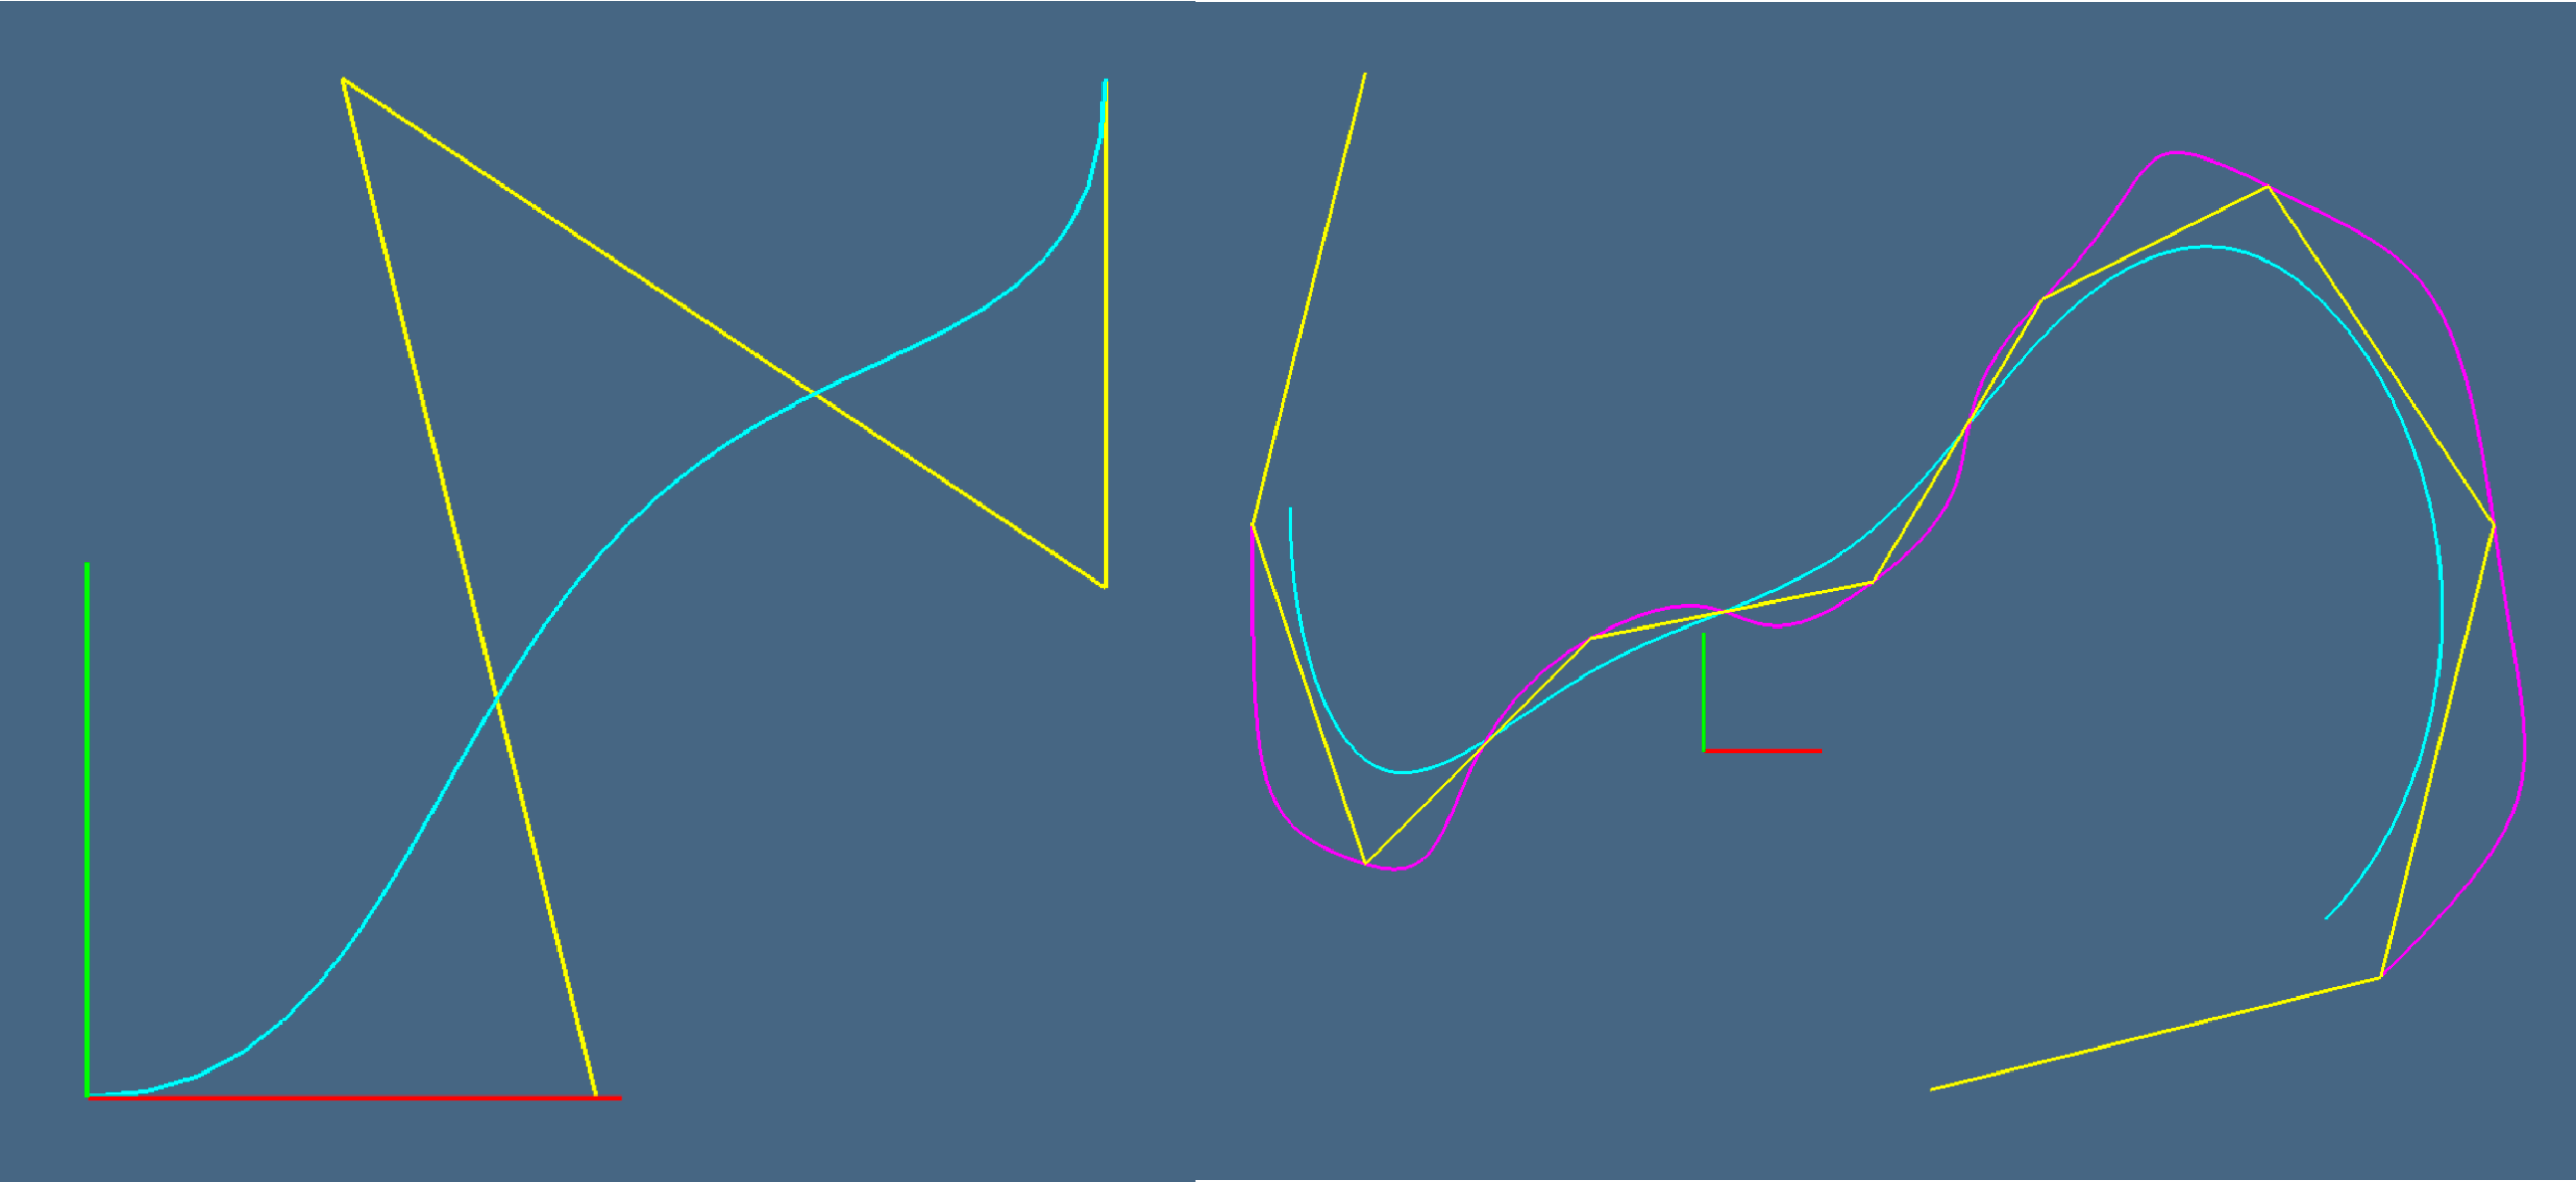
\includegraphics[width=\linewidth]{figs/splinecurves} 
   \caption{(a) Quartic Bézier curve (cyan); (b) splines: cubic cardinal (red); B-spline (cyan) with the same control polygon (yellow)}
   \label{fig:splinecurves}
\end{figure}

\begin{lstlisting}[language = Julia,numbers=none,label={lst:exmpl10},
caption={Spline cardinal and uniform B-spline.}
]
domain = INTERVALS(1.0)(20)
points = [[-3.0,6.0],[-4.0,2.0],[-3.0,-1.0],[-1.0,
	1.0],[1.5,1.5],[3.0,4.0],[5.0,5.0],[7.0,2.0],
	[6.0,-2.0],[2.0,-3.0]]
poly = COLOR(YELLOW)(POLYLINE(points))
cardinal_spline = COLOR(RED)(SPLINE(CUBICCARDINAL(
	domain))(points));
uniform_Bspline = COLOR(CYAN)(SPLINE(CUBICUBSPLINE(
	domain))(points));
VIEW(STRUCT(poly,cardinal_spline,uniform_Bspline))
\end{lstlisting}

Parametric curves can be combined in many ways to create parametric surfaces, solids, or higher-dimensional manifolds. 
Practical classes of surfaces are discussed, in \cite{Paoluzzi2003a}, such as~the \emph{profile product} surfaces, which include rotational surfaces; the \emph{ruled} surfaces, encompassing generalized cylinders and cones; and the surfaces generated by \emph{tensor product} of curves or splines. 
The straightforward combinatorial semantics of the Julia Plasm package may provide valuable insights to the reader with respect to tensor operations and transfinite combinations.

\begin{figure}[htbp] %  figure placement: here, top, bottom, or page
	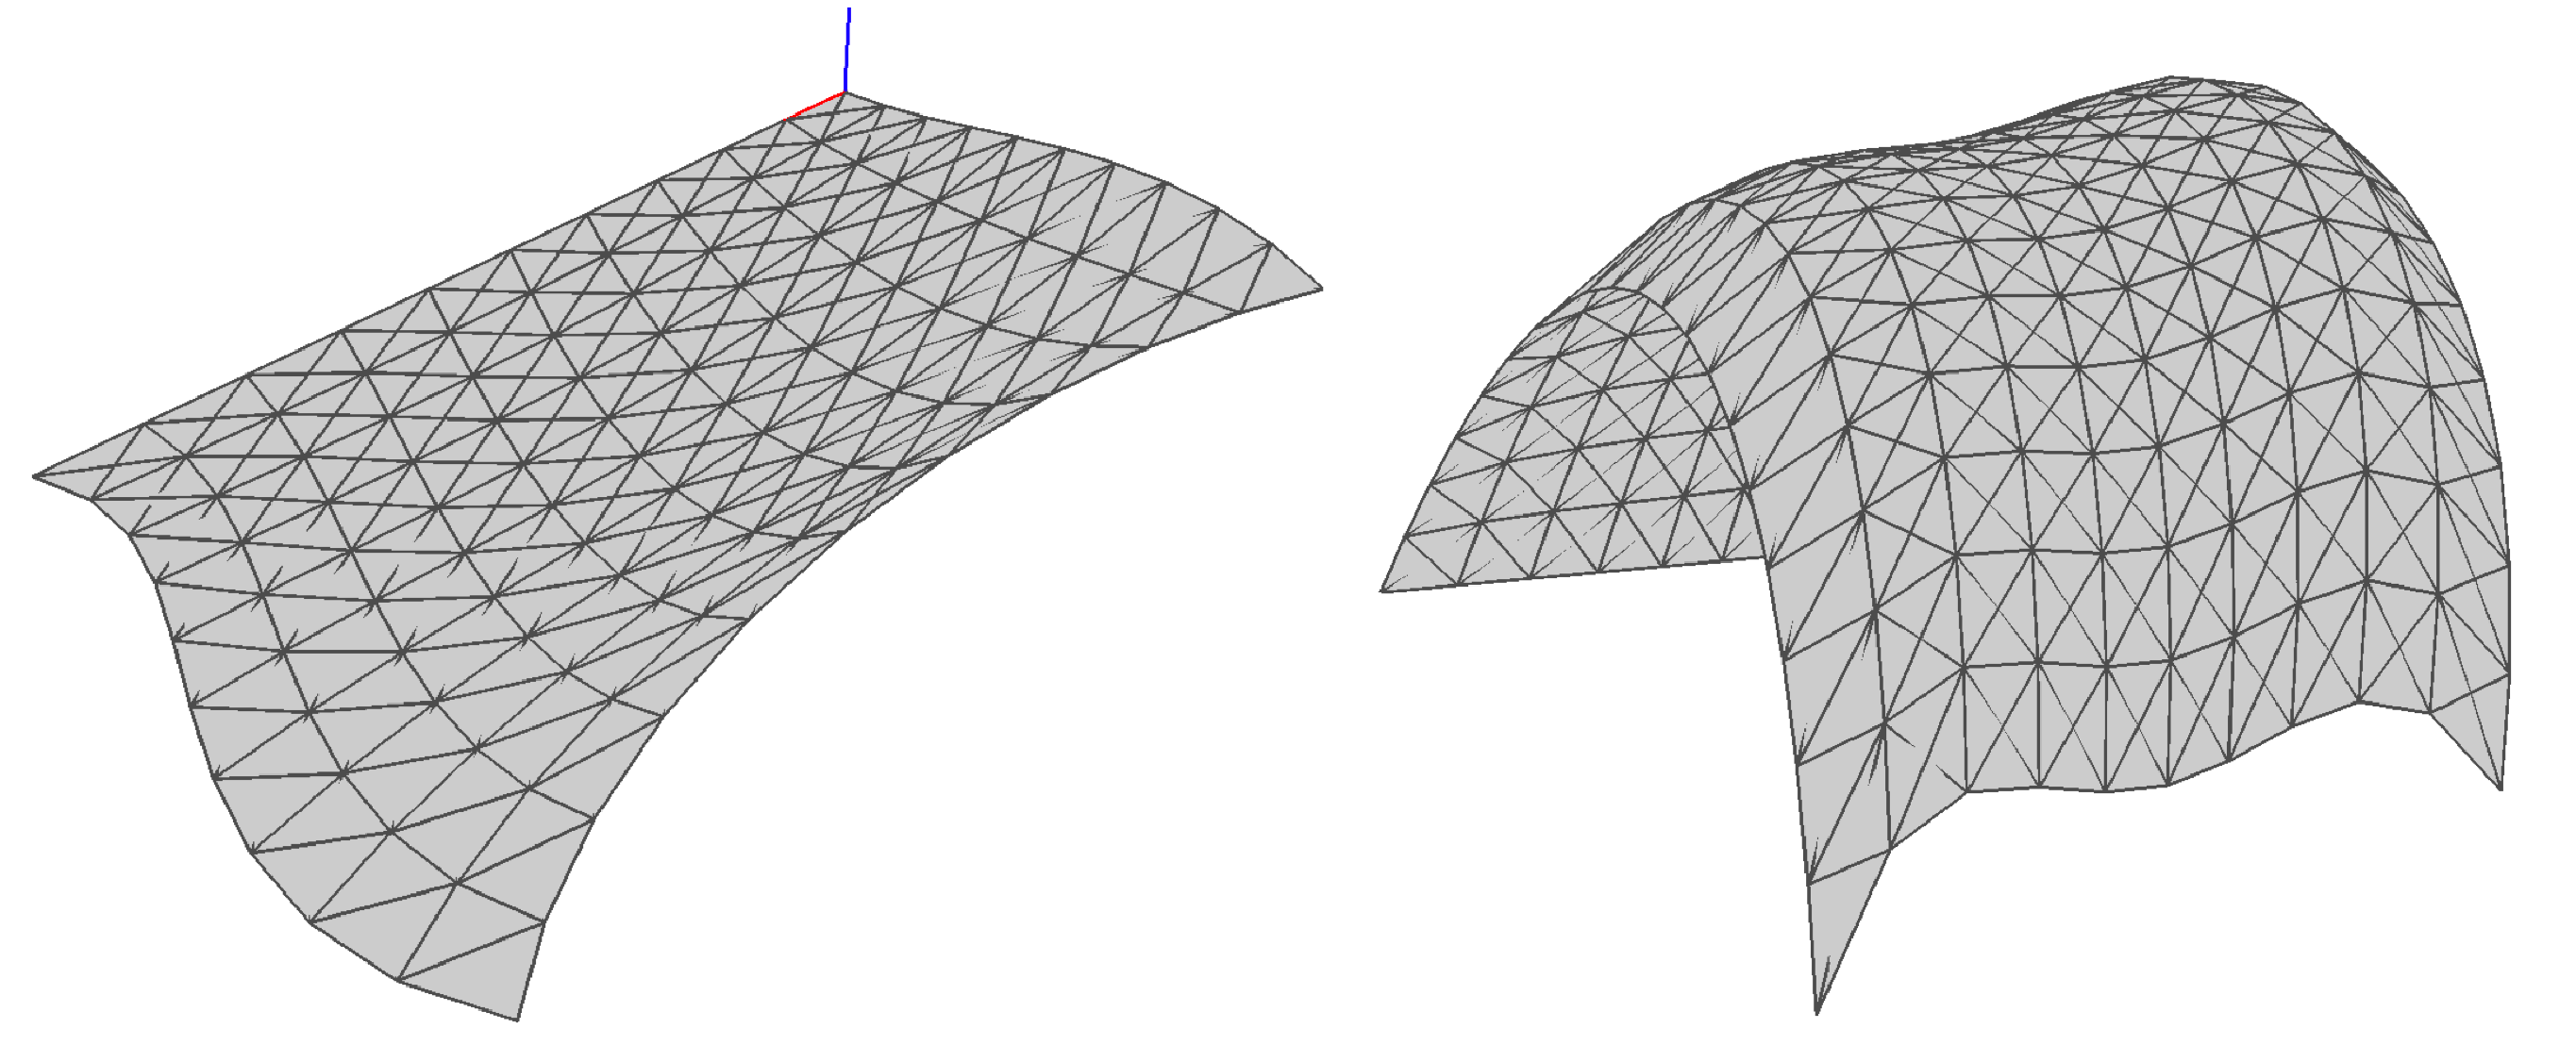
\includegraphics[width=\linewidth]{figs/transfinite}
	\caption{Transfinite surfaces: (a) Bezier surface defined by four different degrees boundary curves; (b) Coons patch defined by four generic boundary curves ({\tt S1, S2} are used to select the {\tt domain} points) first/second coordinate.}
	\label{fig:5:3:transfinite}
\end{figure}


\subsection{Minkowsky operators}
\label{subsec:title_auth}

The  Minkowski sum (or difference) of two convex polyhedra is the convex hull of the points obtained by replicating the vertices of one polyhedron around every vertex of the other one.
Plasm was born multidimensional from the very beginning. Hence, the object representations and the affine transformations, particularly the shearing and the Cartesian products, are dimension-independent. Therefore, exciting and powerful methods for growing the intrinsic dimension of geometrical objects can be defined by bringing them into higher dimensions, then transforming affinely, and finally projecting back into the original embedding space. For example, the object shown in Figure \ref{fig:houseoffset} is appropriately extruded in $\E^6$ space, and then projected back in $\E^3$. 

\begin{lstlisting}[language = Julia,numbers=none,label={lst:exmpl10},
caption={House 3D model by Minkowsky {\tt OFFSET}.}
]
verts = [[0.,0.,0.],[3,0,0],[3,2,0],[0,2,0],[0,0,
	1.5],[3,0,1.5],[3,2,1.5],[0,2,1.5],[0,1,2.2],
	[3,1,2.2]]
cells = [[1,2],[2,3],[3,4],[4,1],[5,6],[6,7],[7,
	8],[8,5],[1,5],[2,6],[3,7],[4,8],[5,9],[8,9],
	[6,10], [7,10],[9,10]]

House = MKPOL(verts, cells)::Hpc
VIEWCOMPLEX( LAR(House) )
VIEWCOMPLEX( LAR(OFFSET([0.2, 0.2, 0.5])(House)) )
\end{lstlisting}
\vspace{-5mm}
\begin{figure}[htbp] %  figure placement: here, top, bottom, or page
   \centering
   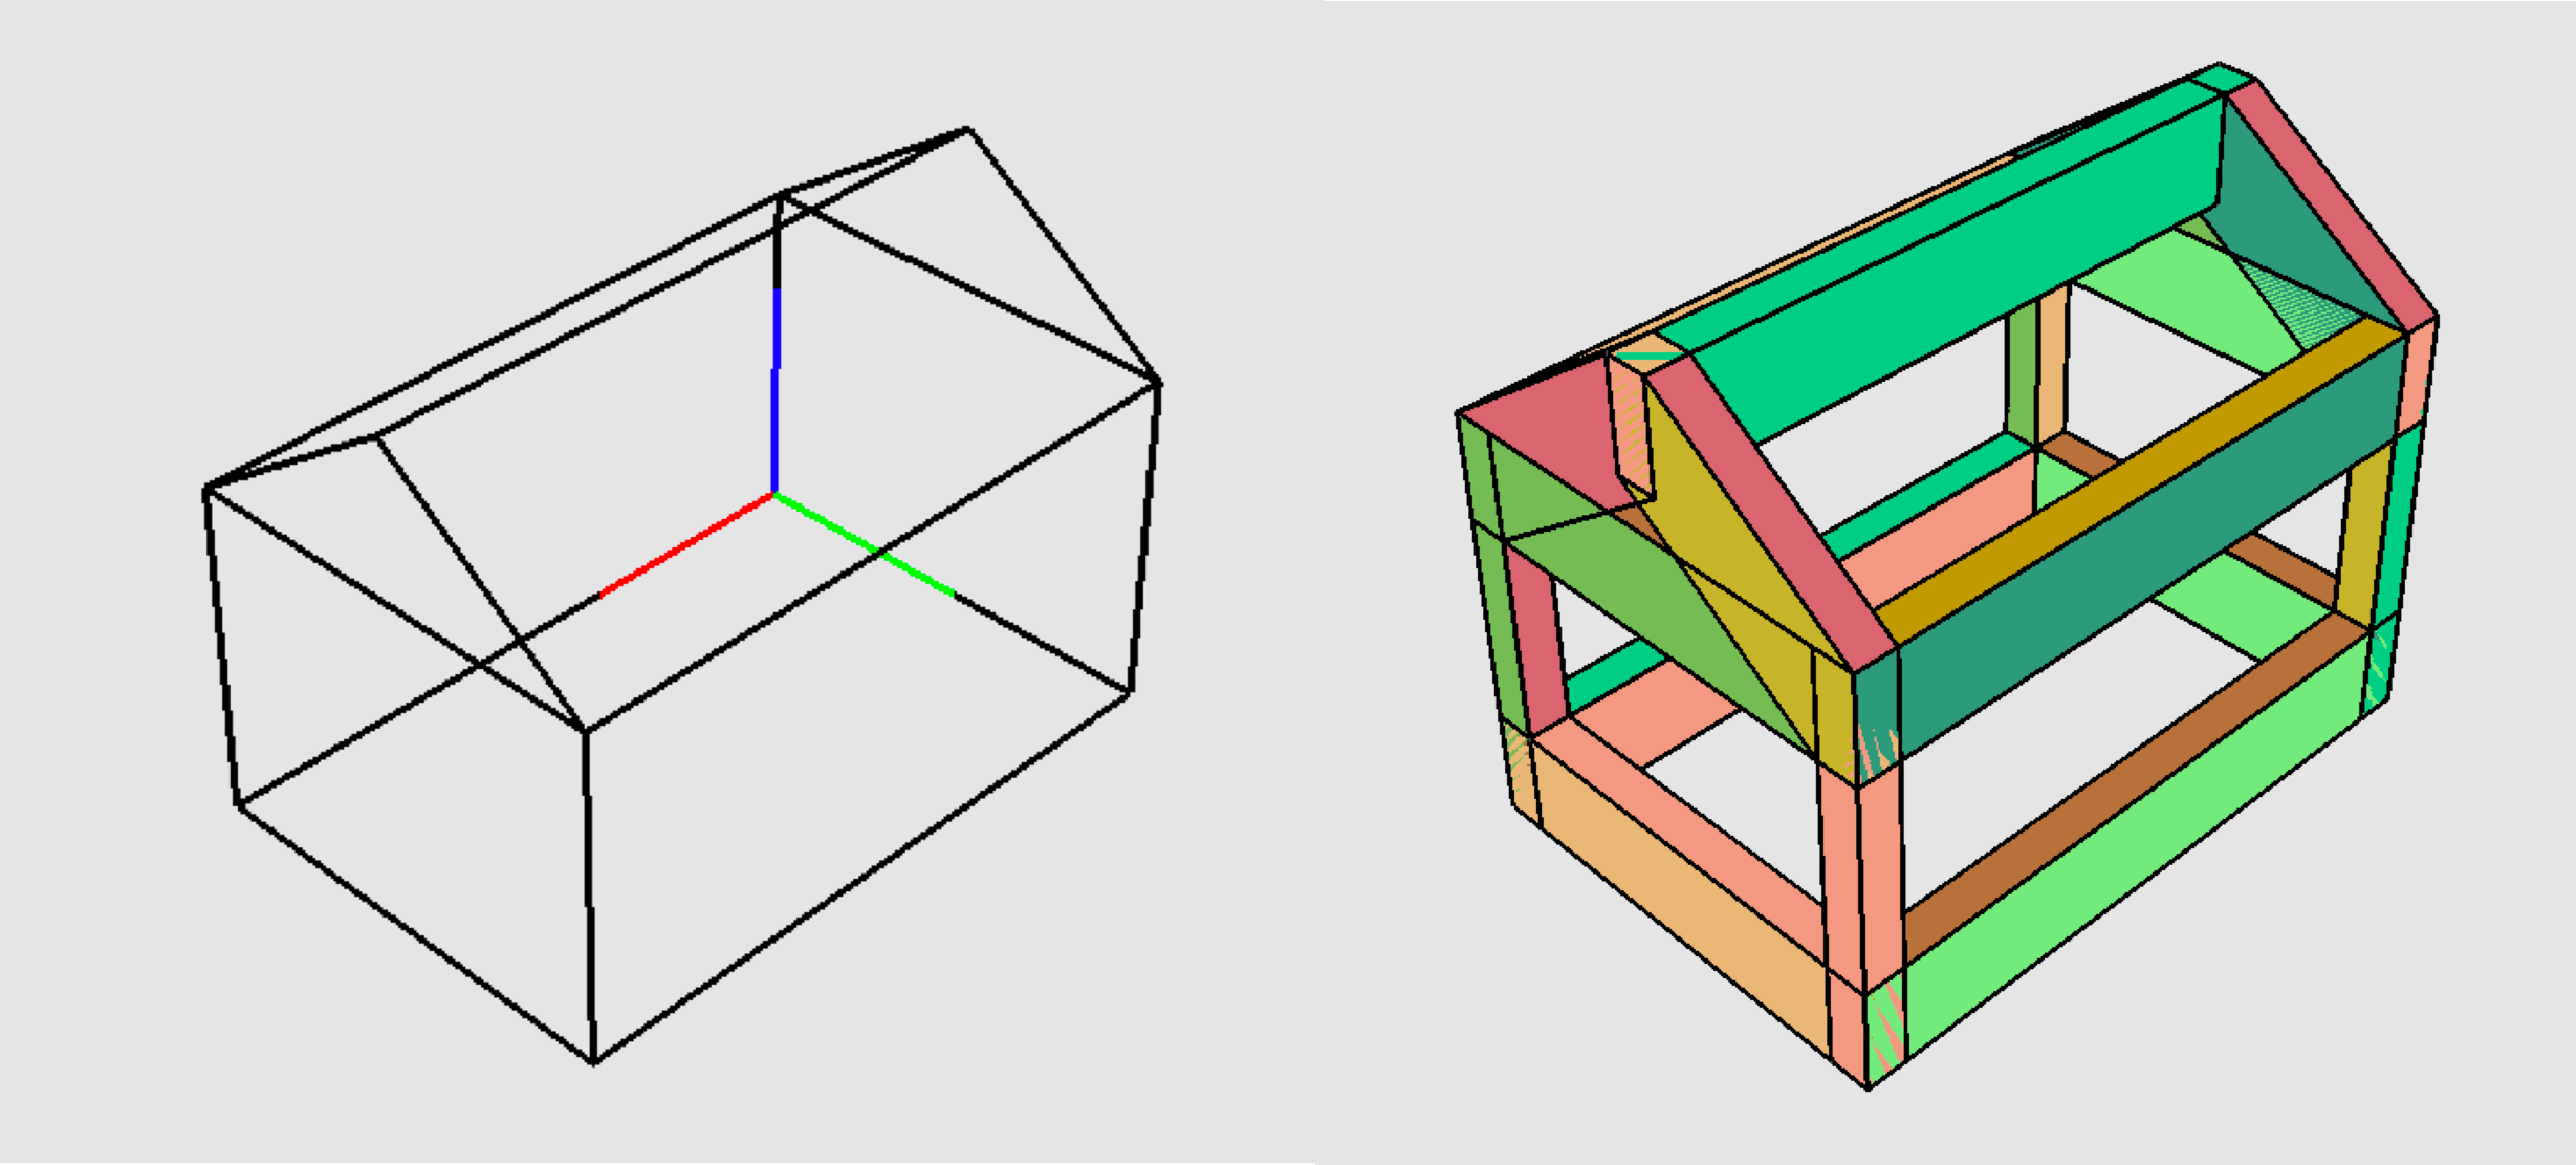
\includegraphics[width=\linewidth]{figs/offset} 
   \caption{(a) Wire-frame geometric model (1-complex) given as a 3D graph in {\tt (verts,cells)}; (b) the generated 3-complex through {\tt OFFSET} operator.}
   \label{fig:houseoffset}
\end{figure}



\subsection{Enumerative schemes and geometric combinators}
\label{subsec:title_auth}
A solid model may be described by enumerating the set of solid cells in some partitioning of the embedding space.  It is possible to distinguish between schemes using sparse Boolean matrices as shape parcel enumerators and schemes based upon hierarchical space decompositions, say \emph{quadtrees} and \emph{octrees}.  Such representations are approximations of the object's space occupancy, even for linear polyhedra. 

\begin{figure}
\centering
	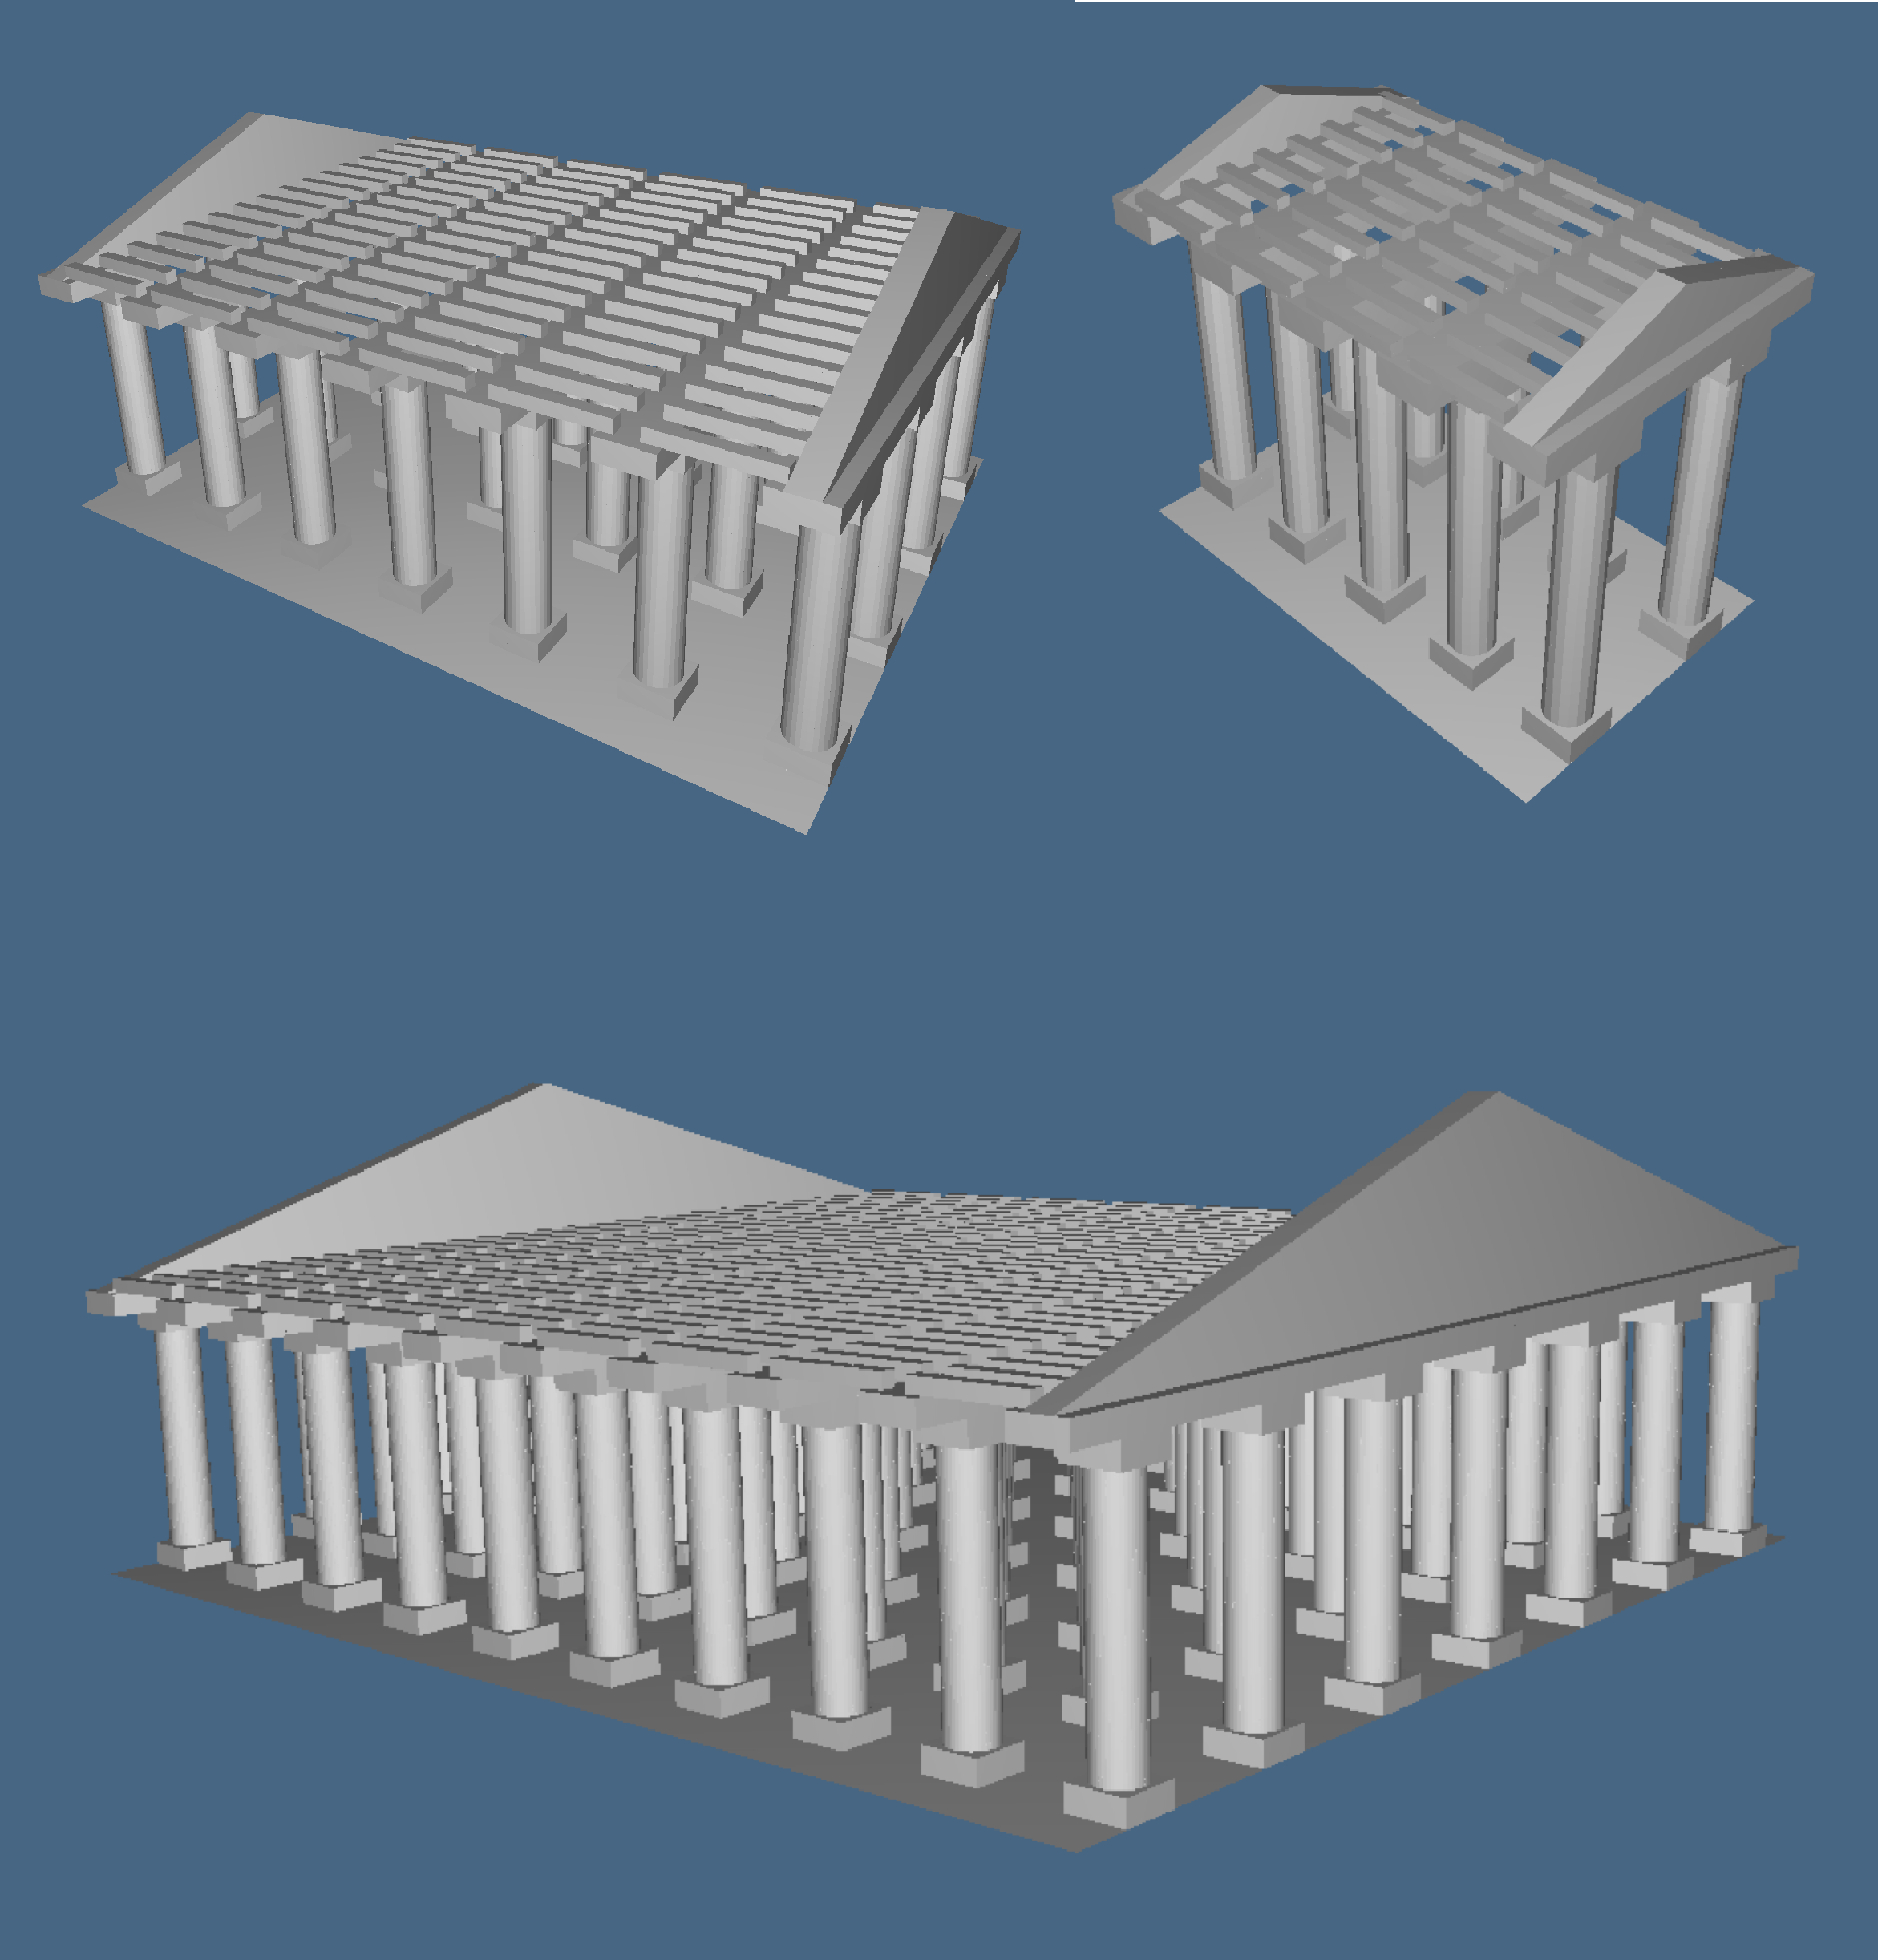
\includegraphics[width=0.5\linewidth]{figs/temples}
	\caption{The fully parameterized {\tt temple()} function features some parameters that are interconnected through algebraic equations. Let’s note the number of side and front columns and their relationship to column height and gable width. Additionally, observe the mixture of 3D and 2D objects, where {\tt PROJECT(2)()} and {\tt BOX(3)(temple)} generate the ground rectangle of the right size.}
	\label{fig:5:temples}
\end{figure}

This scheme is also used in Plasm, e.g., by the {\tt CUBOIDGRID} and {\tt SIMPLEXGRID} generator functions, which accommodate basic topological cells like small cubes or simplices within textured (even curved) shapes used, for example, in 3D printing and new multi-material shapes.

The hierarchical enumerative approach can be simulated in some sense by using the operators {\tt LEFT}, {\tt RIGHT}, {\tt UP}, and {\tt DOWN} in 2D and 3D; {\tt TOP}, and {\tt BOTTOM} in 3D, always between {\tt Hpc} objects, able to be easily converted into graph structures in computer memory. In Plasm, the enumerative scheme may be extended to grids that alternate similar solid shapes and empty intervals of embedding space. This approach would dramatically accelerate the easy and fast development of preliminary design models, mainly in architecture and civil engineering.


\section{Visualization \& interaction platforms}
\label{sec:additional_doc}

The {\tt src/viewer.jl} module of {\tt Plasm.jl} provides an interactive geometry viewer for visualizing and interacting with the shapes generated by the Plasm codes. It supports rendering on a laptop terminal screen and within the HTML interface of a web browser. The web-based viewer was developed to display Plasm models online and facilitate writing rich-text examples and exercises in a web notebook, eliminating the need to install any software.

\subsection{GLFW-based multi-platform 3D viewer}
\label{subsec:title_auth}

As the many examples clearly showed, a geometric computing platform needs powerful and easy methods to visualize and interact with an object’s model under development. Currently, the primitives {\tt VIEW} and {\tt VIEWCOMPLEX} allow the user to present interactive environments with many graphical features, including colors, perspective, and parallel projective presentation.

Two submodules extend this functionality by integrating external libraries. {\tt Viewer.glfw.jl} leverages GLFW, an open-source, multi-platform library for developing OpenGL, OpenGL ES, and Vulkan applications. Meanwhile, {\tt viewer.meshcat.jl} utilizes {\tt MeshCat.jl}, a remotely-controllable 3D platform built on {\tt three.js} library for web applications. {\tt MeshCat.jl} allows local visualization and interaction with Plasm models directly in a web browser, such as within a {\tt Jupyter} notebook controlled by a Julia server, local or remote.

\subsection{Notebook environment execution}
\label{subsec:title_auth}

The platform design includes multiple execution and visualization environments that support different user needs and computational requirements.
With its OpenGL GLFW viewer, the full-featured desktop application enables researchers to access native user interfaces and local computing resources for detailed model interaction and intensive tasks.

But {\tt Plasm.jl} also operates without restrictions in Jupyter notebook environments \cite{JUP}. In this case, the geometric backend communicates to the graphical front-end via a message queue. It renders the results in a simple browser by leveraging its JavaScript engine, which has advanced rendering capabilities and can render even very large geometric models \cite{UP20}.

Julia users of Plasm geometric applications can execute notebooks through either a local machine server or a remote server operating on high-performance computing infrastructure. Furthermore, users benefit from dual-mode accessibility because they can select the most suitable interface and computational backend according to their needs between local analysis and collaborative resource-intensive computations on remote servers.

\subsection{Two-dimensional SVG input}
\label{subsec:title_auth}

Plasm lacks, by design, a graphical user interface, but it can import 2D designs from SVG files. Scalable Vector Graphics (SVG) is the W3C standard for 2D vector graphics on the Web based on XML.  The SVG standard includes support for several primitives, interactive exchange from mouse clicks and touch events, as well as animated visualization in response to user actions. The primitives can be filled with color or a gradient. The wireframe drawing (stroke) can also be rendered with a specific width, possibly using solid Plasm primitives. Some features will be ported to Plasm in a future version. 

To extend Plasm's capabilities with Scalable Vector Graphics (SVG) support, we developed a Julia parsing module that processes SVG files by (*) parsing the XML structure using the XML.jl library [XML], (*) traversing the XML tree, and applying systematically and accumulating transformations to ensure all graphical elements are embedded in a global coordinate space.

All the core SVG shapes (e.g., rectangles, circles, ellipses, lines, polylines, polygons) and complex path data are converted into standardized polyline or polygon representations. For curved elements (including path segments like Bezier curves and elliptical arcs) user can set a configurable number of points to sample and generate the polyline approximation.

\begin{figure}[htbp]
	\label{fig:7:2:svg2}
    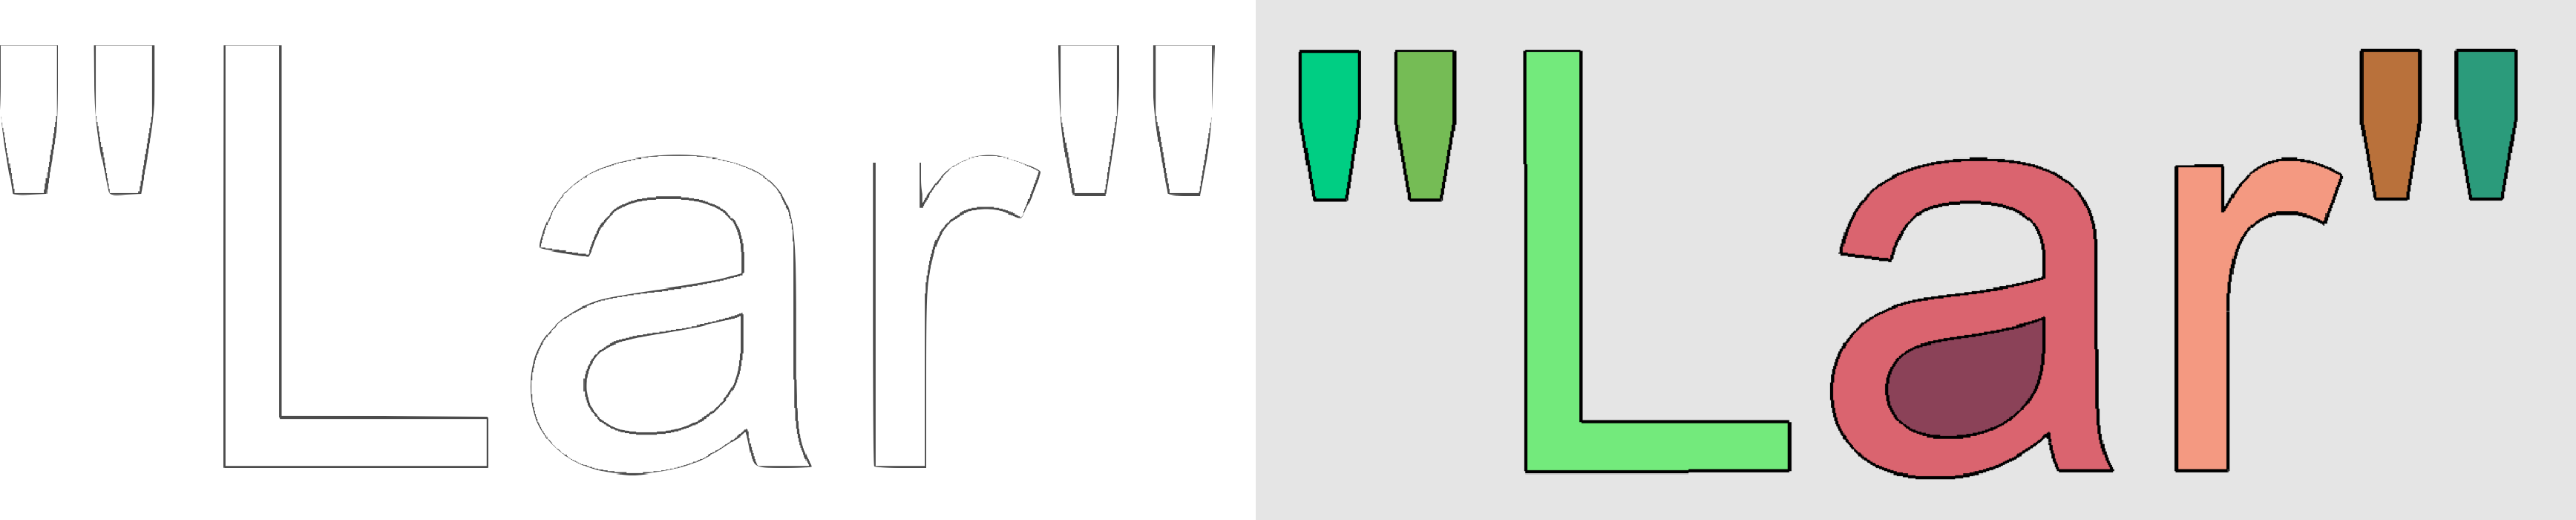
\includegraphics[width=\linewidth]{figs/two-Lar.pdf}
    \caption{Images generated by {\tt Plasm}: (a) one-dimensional {\tt Hpc} model generated by the expression {\tt SVG(“filename.svg”)}. Note that the model of the {\tt "Lar"} string includes several curved splines; (b) atoms in different colors generated by {\tt ARRANGE2D} primitive. The {\tt outer} atom and cell (irreducible to a point, see Section \ref{}) is the ivory background.}
\end{figure}

The parser also tries to preserve the most important style attributes, including fill color, stroke color, and stroke width, to store in {\tt Properties} field of data objects. Color definitions, whether specified as hexadecimal values, RGB/RGBA functions, or named colors, are consistently converted into four-component RGBA (Red, Green, Blue, Alpha) arrays, thus facilitating their direct use in subsequent rendering or analysis pipelines within Plasm.

For the polygon PL-filling from low-degree spline curves, we provided in-house using the classic PLaSM algorithm \cite{Paoluzzi2003a} with Boolean {\tt XOR} of planar adjacent stripes generated by the polygon profile of a spline curve. Of course, the {\tt src/pdf/} module contains the initial development stage and requires much more work, extensive testing, and time.

Importing and parsing {\tt .svg} files generated by interactive design environments and stored in local memory or the cloud is a crucial link between the Plasm language running the {\tt REPL} interpreter on a local or remote terminal and the CAD extrusion of file content. At present, we have only performed a few experiments interfacing the geometric language with this web tool, but it is considered a high-priority project for the {\tt Plasm} platform.


\subsection{PLY format reading and writing}
\label{subsec:title_auth}

To enhance its versatility and facilitate the integration of existing 3D assets, Plasm.jl allows importing external geometric models using the Polygon File Format (PLY) 
\cite{mathworks-ply-format}. The PLY format is a common standard for representing 3D data, mainly originating from 3D scanners or other modeling software. PLY support allows users to bring these external geometries into the Julia computational environment.

First, we parse {.ply} files to extract essential geometric information, including vertex coordinates and face definitions. After reading this raw data, {Plasm.jl} translates it into internal data structures, typically the form of cellular complex provided by the Julia Plasm {\tt Lar} data type. This conversion process ensures that the imported model, regardless of its origin, is represented in a manner consistent and compatible with {\tt Plasm.jl}’s native geometric objects, allowing further elaboration.

By transforming external data into its internal format, the Julia Plasm package allows users to import models obtained from a wide variety of sources, significantly extending the platform's interoperability and practical application scope in research and development workflows involving pre-existing 3D datasets.


\section{Arrangements and Boolean Algebra}
\label{sec:additional_doc}

This section synthesizes the Plasm innovative approach to the Boolean algebra of solid models, rooted in the algebraic topology of piecewise-linear geometry. Specifically, Plasm implements computational topology algorithms to uncover the two- or three-dimensional space partitions (called arrangement by combinatorial topologists) formed by collections of 1D and 2D geometric objects, respectively \cite{Plasm:book:2005}.

Julia’s sparse arrays, with their standard algebraic operations, were the principal data types for our computational program. Their extensive use \cite{TSAS:2020} for topology representation allowed us to handle general cellular complexes that are homeomorphic to $d$-polyhedra, representing triangulable spaces that can be non-convex and multiply connected.

Sparse arrays, with their standard algebraic operations, were essential data structures for our computational program. They permitted us to handle general cellular complexes homeomorphic to $d$-polyhedra, representing triangulable spaces that can be non-convex and multiply connected. The computation of \emph{space arrangements} was the preliminary step toward generating Boolean solid algebras and the binary resolution of any Boolean expression within.

\subsection{Space homology pipeline}
\label{subsec:title_auth}

To clarify, it may be beneficial to revise the mathematical notation for “chain complex”, which we restate here with our data structure notation for the user’s convenience. For sake of reader comprehensibility with respect to the mathematics, we translate the names of sparse matrices of topological operators, and use {\tt EV: V $\to$ E}, {\tt FE: E $\to$ F}, and {\tt CF: F $\to$ C}, with relational meanings from our topological operators ({\tt V, E, F, C} stand for vertices, edges, faces, and cells, respectively).
\[ 
	C_\bullet = (C_p, \partial_p) := 
	C_3 \ 
	\substack{
		\delta_2 \\
		\longleftarrow \\[-1mm]
		\longrightarrow \\
		\partial_3 
	}
	\ C_2 \ 
	\substack{
		\delta_1 \\
		\longleftarrow \\[-1mm]
		\longrightarrow \\
		\partial_2 
	}
	\ C_1 \ 
	\substack{
		\delta_0 \\
		\longleftarrow \\[-1mm]
		\longrightarrow \\
		\partial_1 
	}
	\ C_0 
	\]
	\[
	{\tt C} \ 
	\substack{
		{\tt CF}\\
		\longleftarrow \\[-1mm]
		\longrightarrow \\
		{\tt FC}
	}
	\ {\tt F} \ 
	\substack{
		{\tt FE}\\
		\longleftarrow \\[-1mm]
		\longrightarrow \\
		{\tt EF}
	}
	\ {\tt E} \ 
	\substack{
		{\tt EV}\\
		\longleftarrow \\[-1mm]
		\longrightarrow \\
		{\tt VE}
	}
	\ {\tt V}.
\]


%\begin{figure}[htbp] %  figure placement: here, top, bottom, or page
%	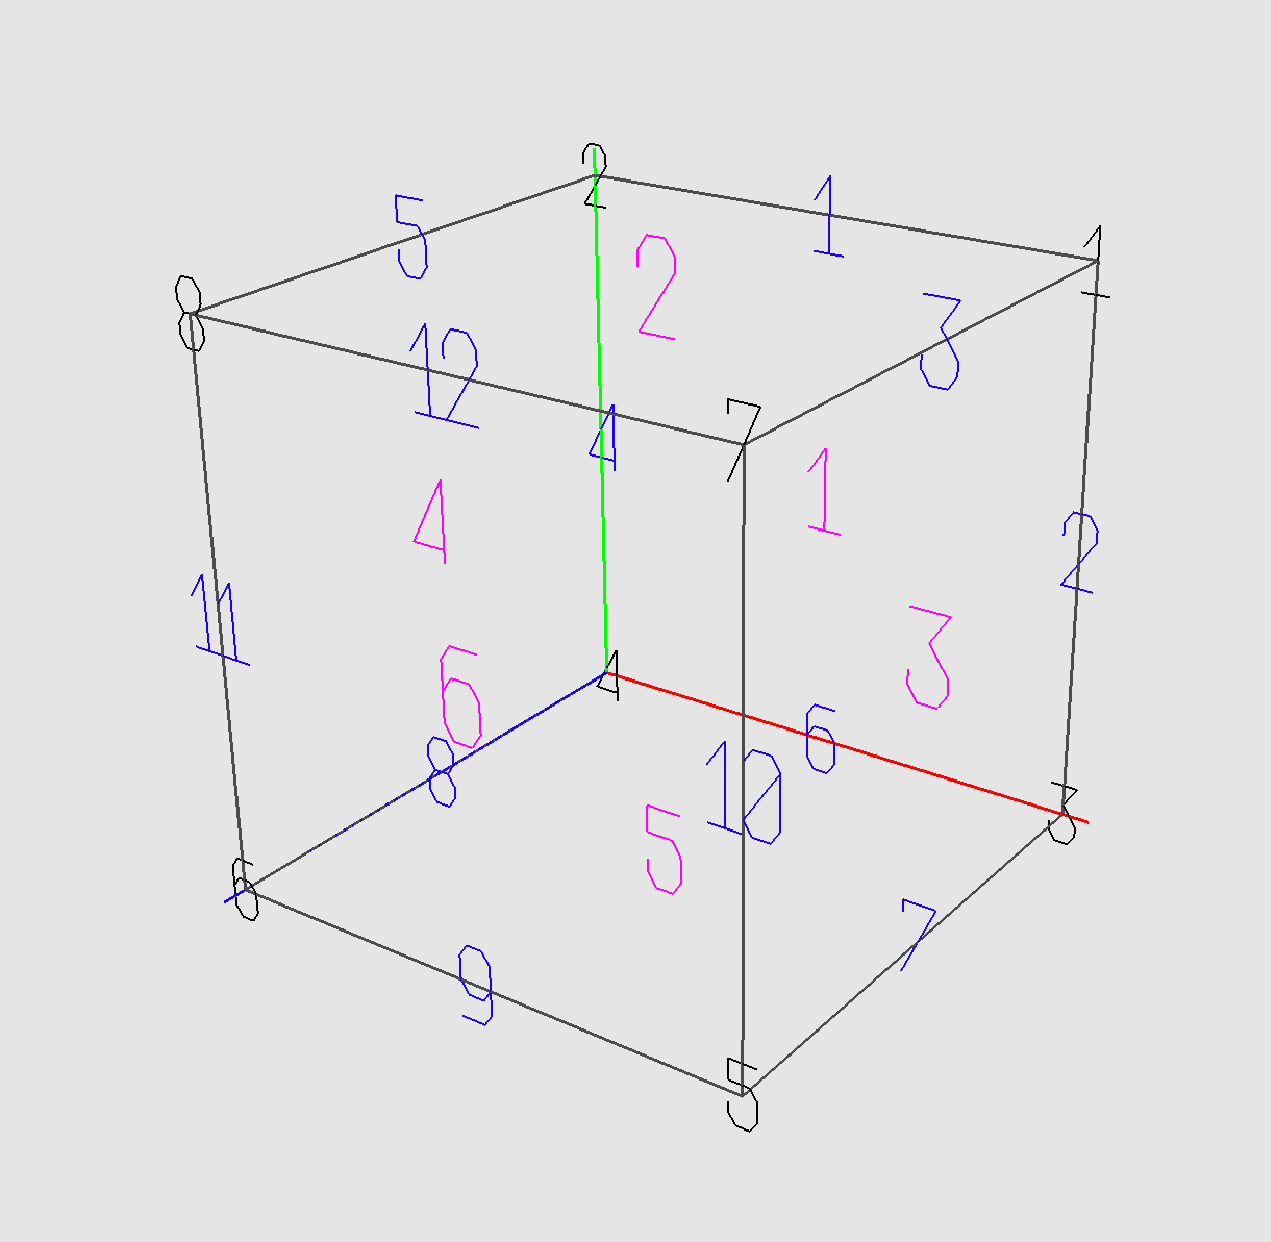
\includegraphics[width=0.35\linewidth]{figs/newcube}
%	\caption{The numbered unit 3-cube cellular complex.
%		The ordinal numbers for vertices, edges, and faces are set in the middle of each 0-, 1-, and 2-cell. Note that the indexes have lexicographic and not geometric order (say, clockwise or counterclockwise), but this is not a constraint. }
%	\label{fig:5:1:cube}
%\end{figure}

Many 2D unit tests have been run during the development and the Plasm implementation of 2D and 3D algorithmic pipelines. In Figure~\ref{fig:6:4:arrange2d}, we show two executions with fifteen squares with random rotation centers (the left-bottom vertex) and angles.
	\begin{figure}[htbp]  \centering
		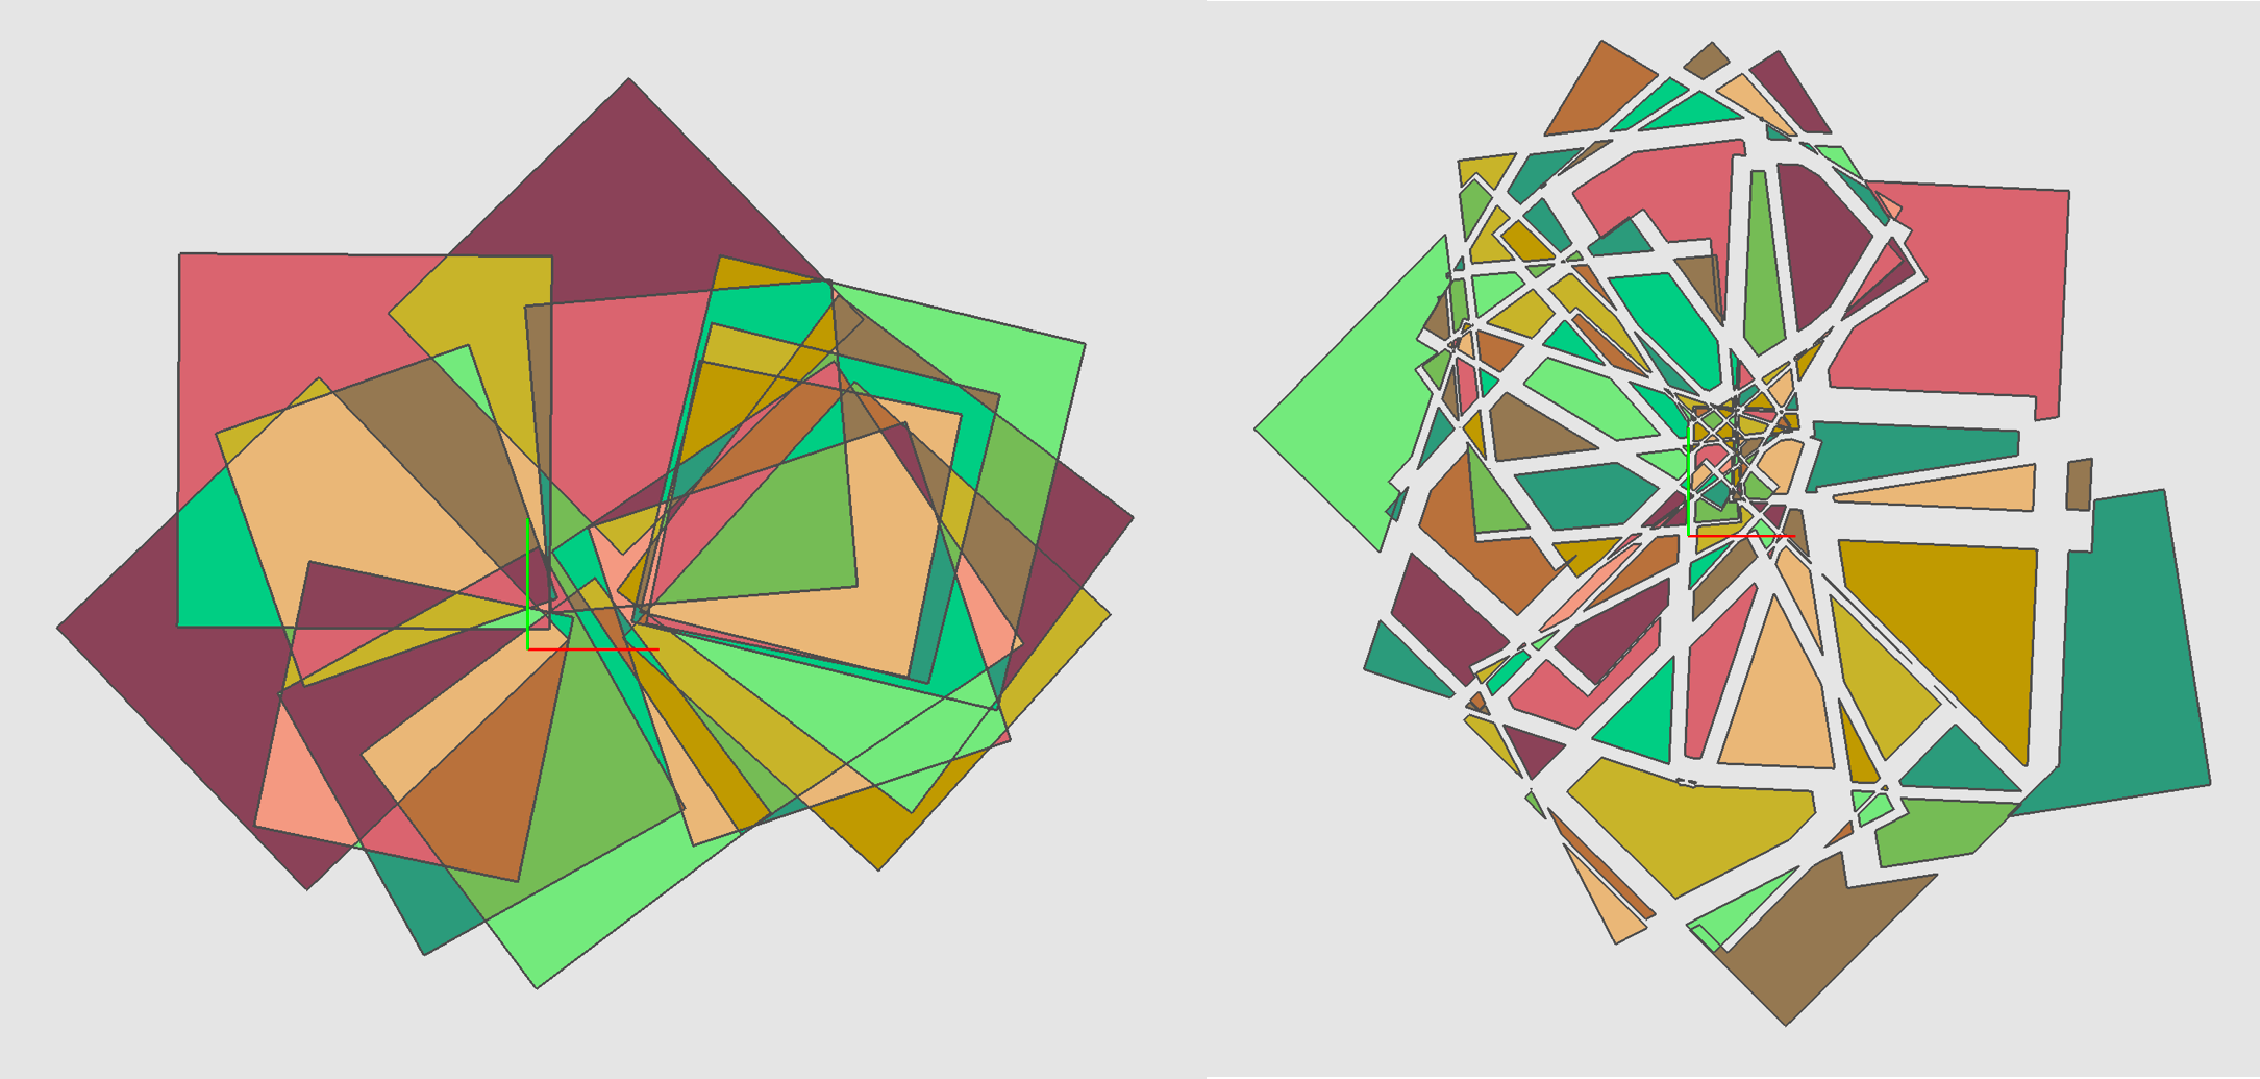
\includegraphics[width=\linewidth]{figs/arrange2d}
		\caption{2D arrangements of two random sets of squares : (a) arrangement atoms in different colors; 
		(b) atoms exploded about the origin.}
		\label{fig:6:4:arrange2d}
	\end{figure}

Similar test examples were developed for implementing the {\tt ARRANGE3D} function, which was later joined with the companion {\tt ARRANGE2D} function into a single {\tt ARRANGE} operator used within the computational Julia Plasm environment {\tt BOOL} to evaluate Boolean solid formulas in 2D or 3D. 

\begin{figure}[htbp]  \centering
	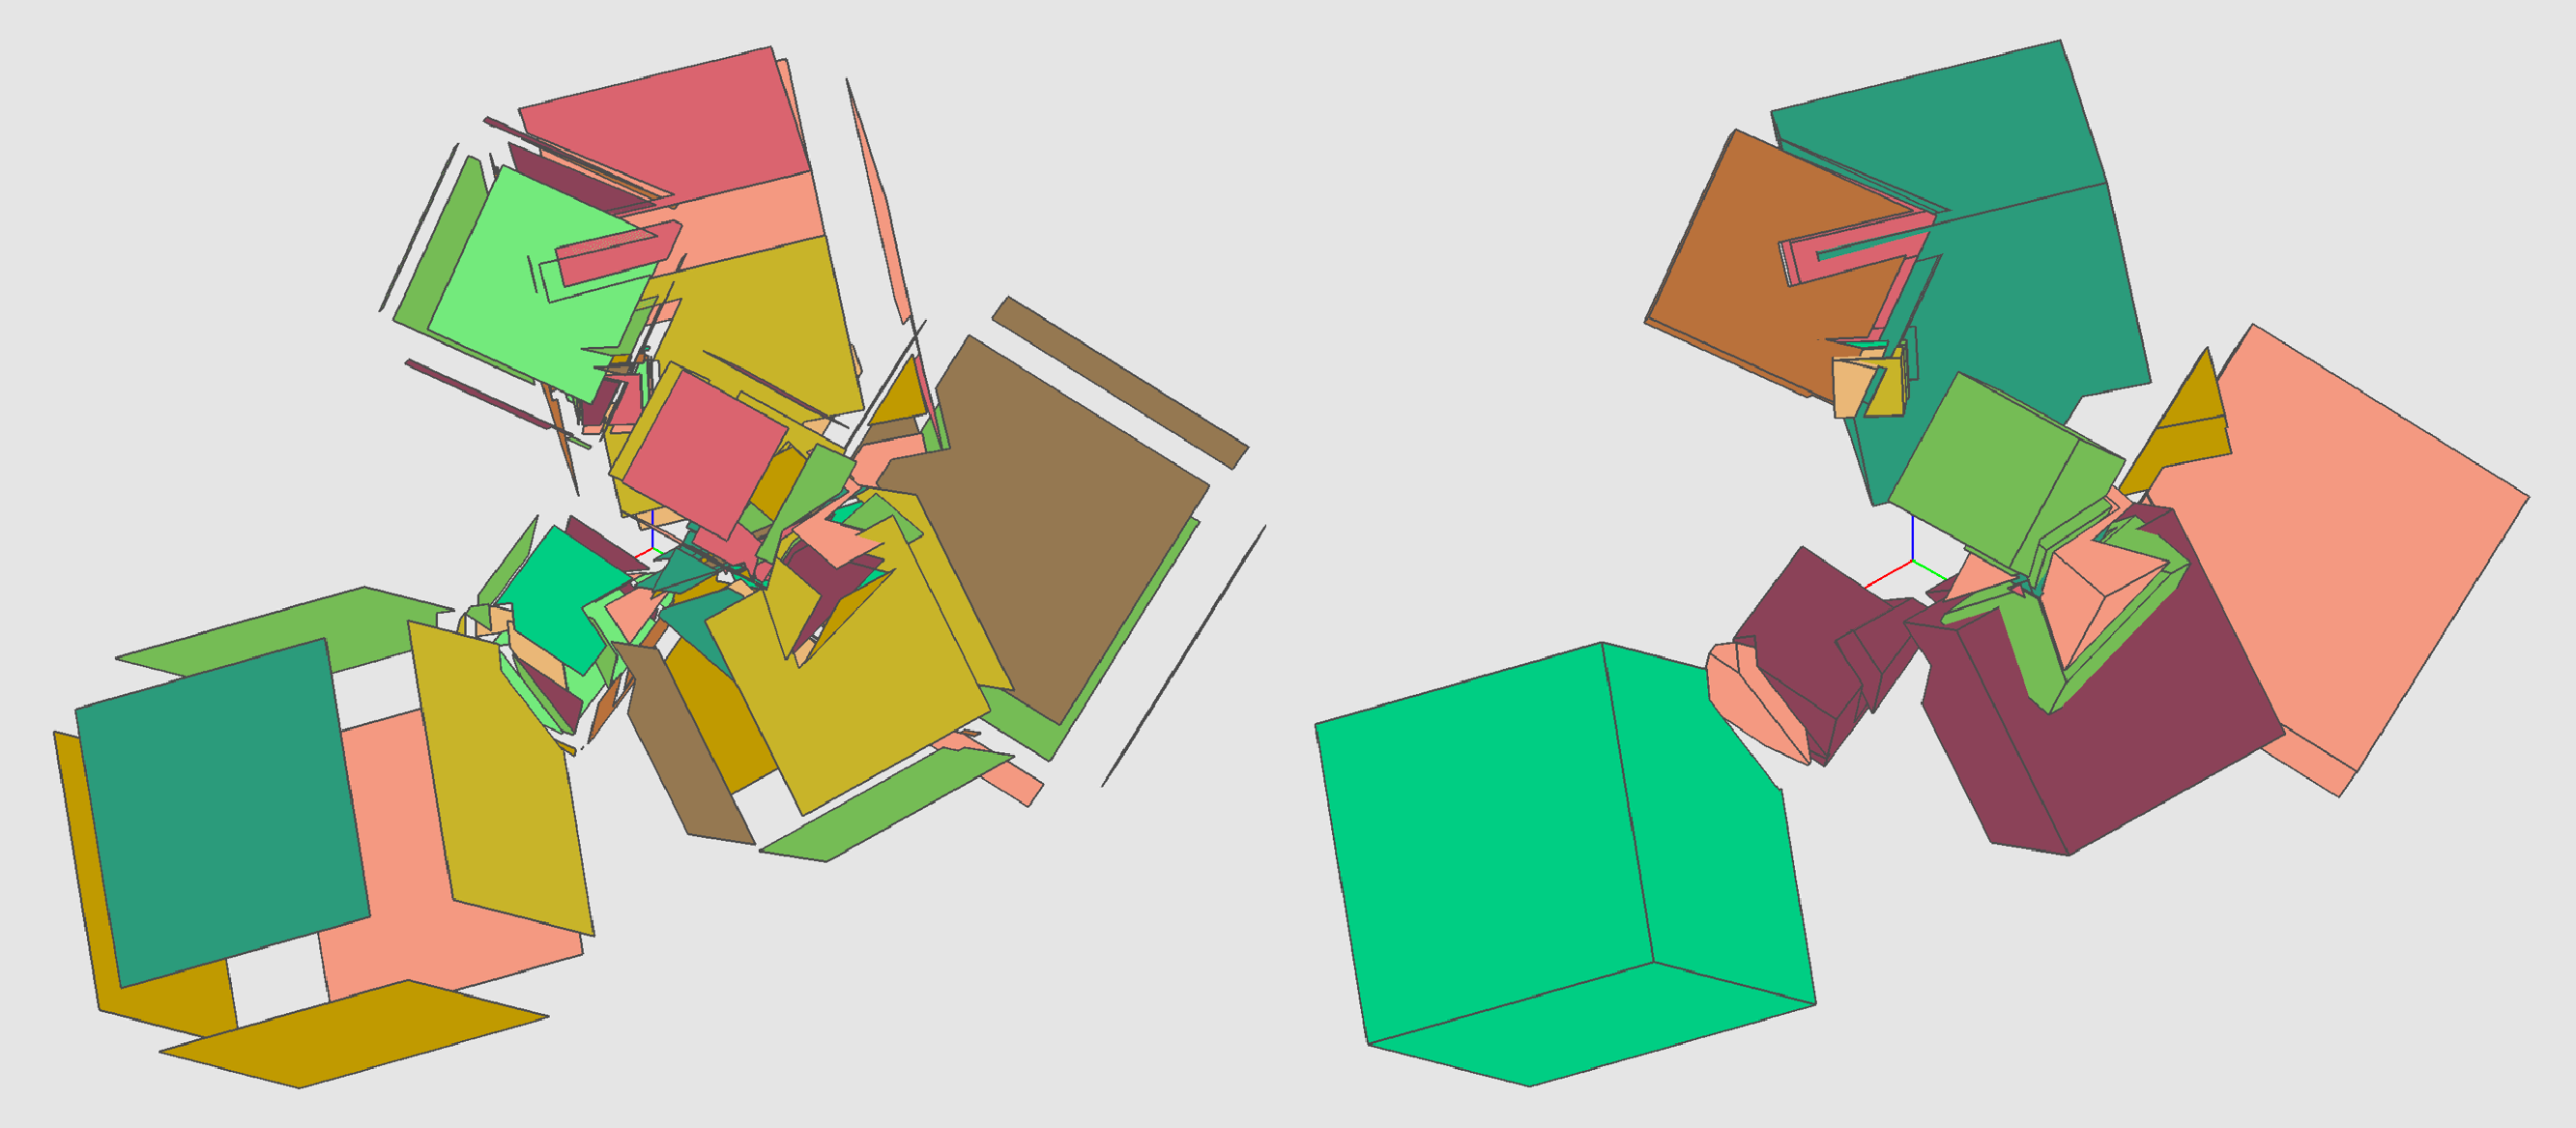
\includegraphics[width=\linewidth]{figs/arrange3d}
	\caption{3D arrangements of ten random cubes: (a) 2-cells of the arrangement atoms; (b) atoms in different colors exploded about the origin.}
	\label{fig:6:4:arrange3d}
\end{figure}



\begin{lstlisting}[language = Julia,numbers=none,label={lst:exmpl10},
caption={aaaa.}
]
hpc = STRUCT([RandomBubble() for I in 1:50])
arrangement = ARRANGE2D(LAR(hpc))
VIEWCOMPLEX(arrangement)
VIEWCOMPLEX(arrangement, explode=[1.5,1.5,1.5])
\end{lstlisting}
	In the above script, we have shown the typical pattern needed for this purpose. First, the set of generators, in this case, 50 random polygons, is correctly assembled within a {\tt Hpc}
	{\tt STRUCT} collection; then it is transformed into a {\tt Lar} cellular complex and passed as an argument to the functions {\tt ARRANGE2D} or {\tt ARRANGE3D} in case of three-dimensional dataset, producing all the atoms of the {\tt arrangement} partition. 
\begin{figure}[htbp]  \centering
	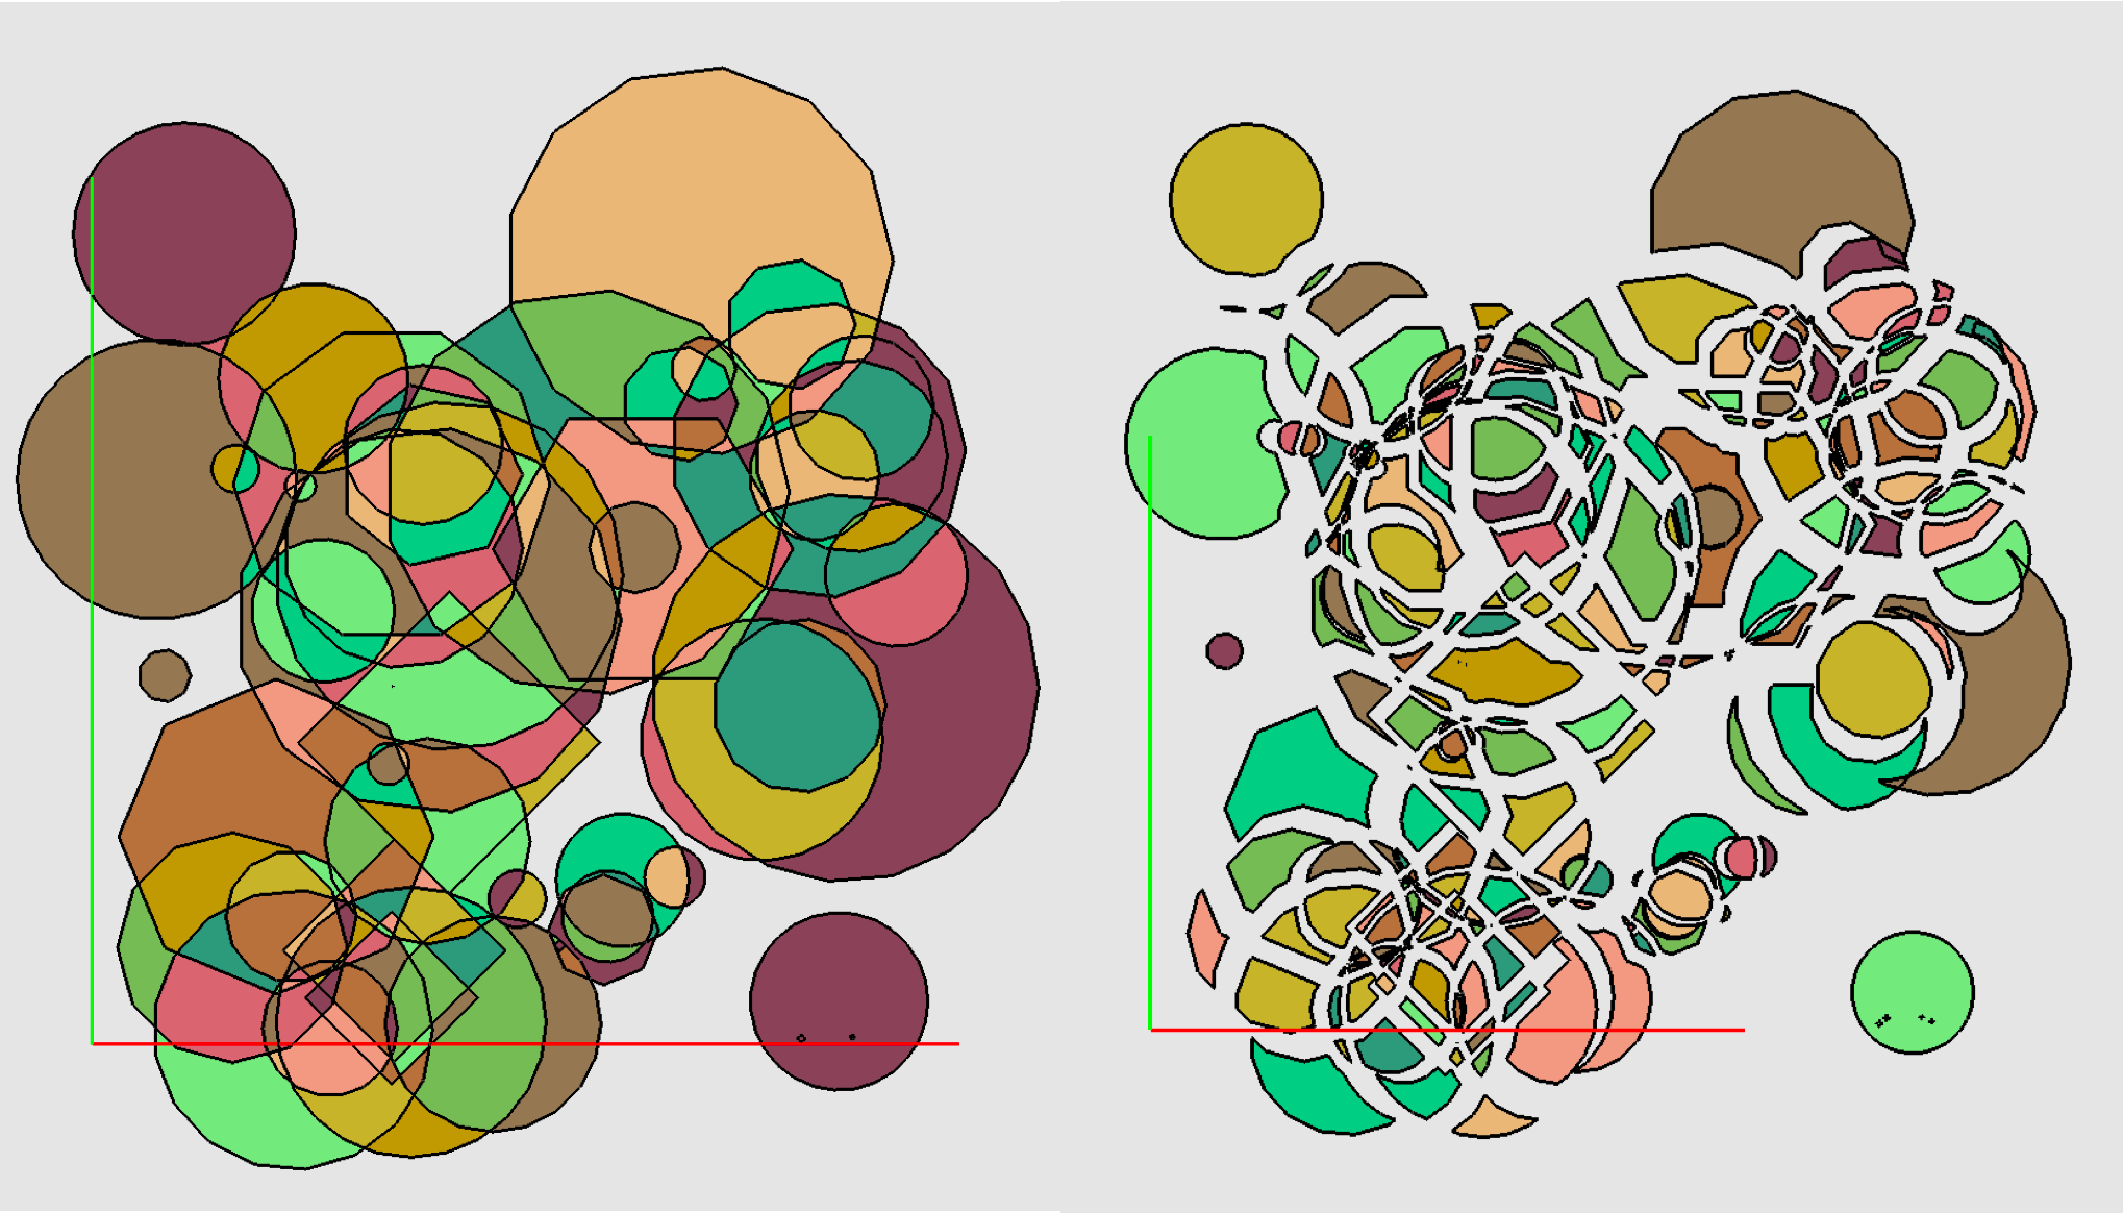
\includegraphics[width=\linewidth]{figs/bubbles}
	\caption{2D arrangements of 50 random convex polygons: (a) 2-cells of the arrangement atoms; (b) atoms in different colors exploded about the origin.}
	\label{fig:6:4:arrange3d}
\end{figure}

	
%\begin{figure}[h]
%		\label{fig:6:TSAS}
%		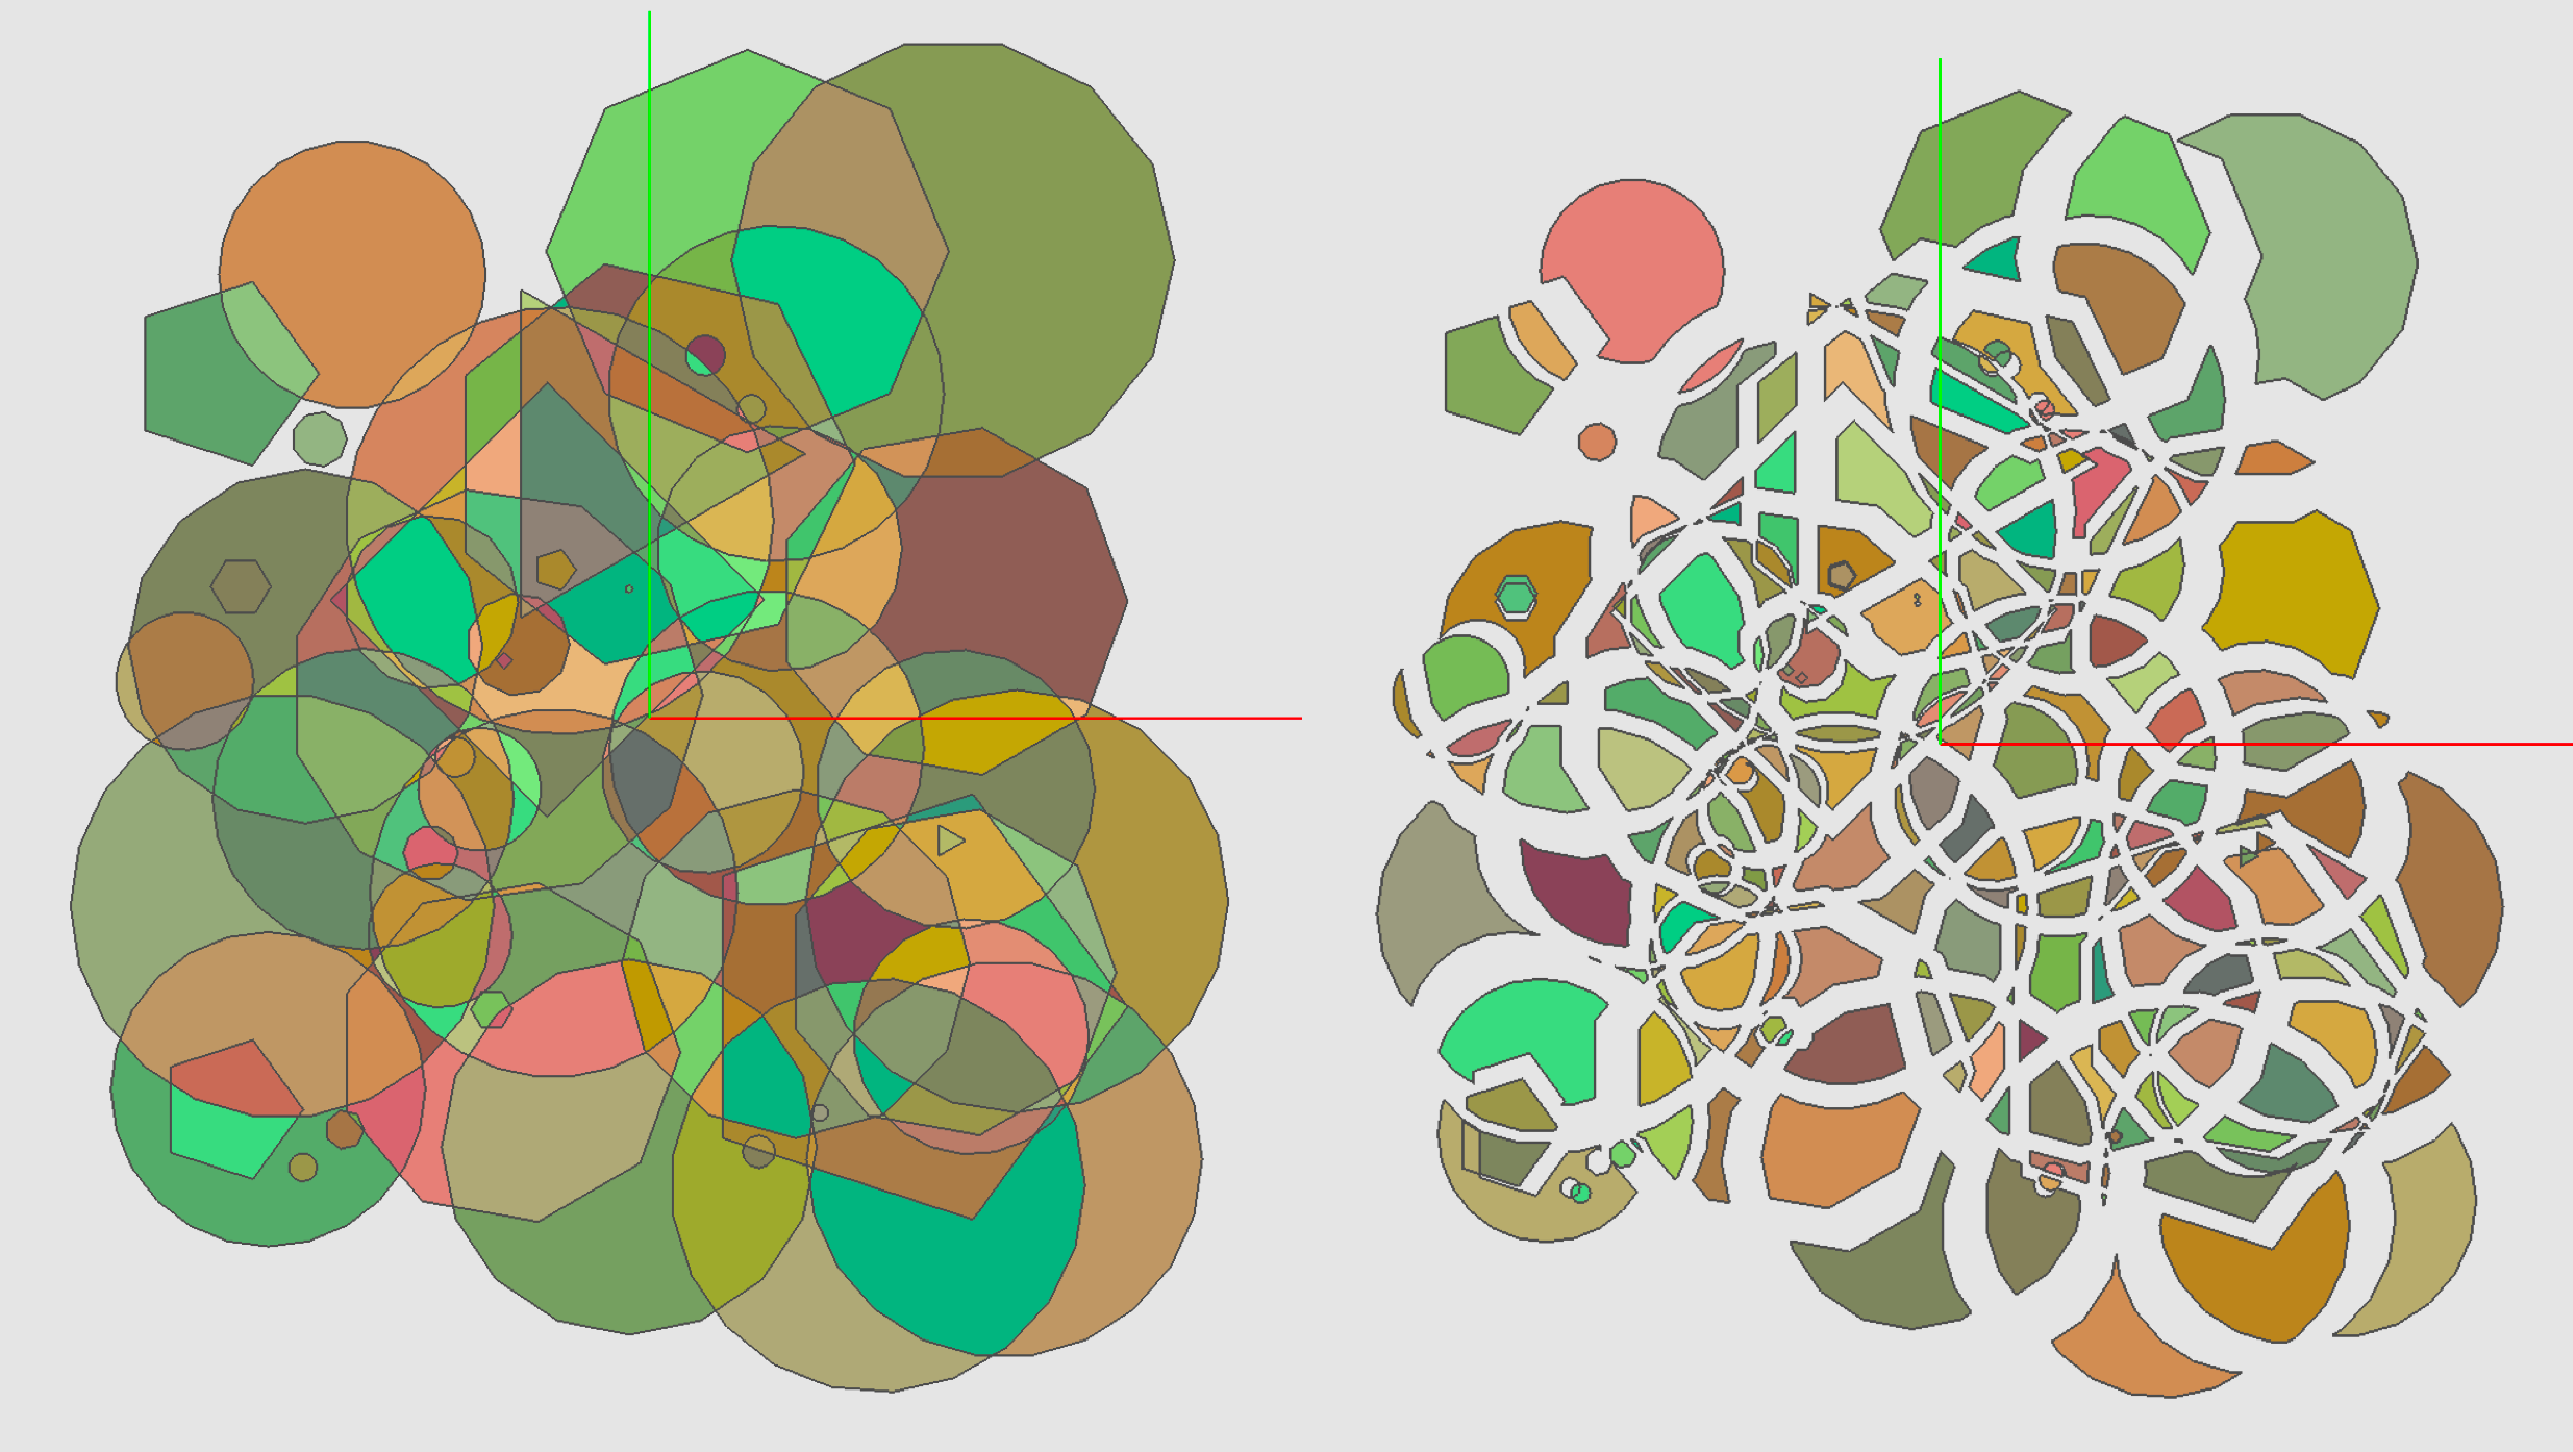
\includegraphics[width=\linewidth]{figs/circles2d}
%		\caption{$\E^2$ arrangement with random polygons: (a)~basis 2-chain $U_2 \subset C_2$; (b) Exploded cell complex. {\tt LAR} cells are neither convex nor contractible.}
%\end{figure}

\subsection{Object generators and atoms}
\label{subsec:title_auth}

\emph{Chain complexes} are an algebraic tool for computing or defining homology. They are used here to algebraically describe a partition of the embedding space induced by a collection of geometric objects, particularly all the cycles (holes) in the dimensions of interest—specifically, from dimension 0 to dimension 3. 

For example, let us consider a building with many \emph{hollow spaces} and thin separation surfaces. Architects and engineers have always designed the structure of internal spaces by creating their separation elements and how they relate. In Plasm, we consider the topological abstraction of incidence and adjacency of elementary separation parts by a sequence of spaces of chains (subsets of cells) and linear operators, so fetching the algebraic tool of a chain complex.

In a Boolean algebra, atoms and generators have distinct roles and definitions. 
In summary, atoms are distinct elements related to the structure and cardinality of Boolean algebra, while generators are elements used to construct or describe this algebra. When considering Boolean strings of finite Boolean algebras, atoms contain only one non-zero element.


	{\tt Plasm} may utilize via the {\tt Lar} type very general 2-cells, possibly non-convex and featuring holes. Refer to Figure \ref{fig:twocubes2}b. It’s important to note that the {\tt partition} object includes all the 3D atoms of the $\E^3$ arrangement generated by the {\tt Plasm} expression {\tt ARRANGE3D(LAR(hpc))} including the holes present in the embedding space $\E^3$. 
	
Conversely, {\tt INNERS(partition)} comprises only the atoms (inners) that do not contribute to the finite boundary of the exterior unbounded atoms {\tt OUTERS(partition)}. In our scenario, this collection is connected and cannot be exploded by {\tt Plasm}; therefore, only one hole exists in the exterior 3D space. 

\subsection{Boolean solid algebras}
\label{subsec:title_auth}

\subsubsection*{The fundamental property}\label{sec:traversal}
\index{Algebra!finite!} 

At the core of the Boolean operations between solid rigid models implemented in our {\tt Plasm} language, there is the following fundamental property:
\index{Algebra!finite!} 

\begin{property}[Boolean atoms are unit 3-chains]
    There is a \emph{natural transformation} \footnote{In category theory, a branch of abstract mathematics, a \emph{natural transformation} provides a way of transforming one functor into another while respecting the internal structure (i.e., the composition of morphisms) of the categories involved. Hence, a natural transformation can be considered a "morphism of functors.”} between $d$-chains defined on a spatial arrangement and the solid algebra generated by that arrangement. 
\end{property}

Solid objects are often defined as hierarchical assemblies of solid primitives or more complex shapes, each represented in a local coordinate system. 
Most graphics and modeling systems implement this semantics as a hierarchical graph, where affine geometry within the nodes is defined in local systems. Arcs are linked to affine transformations that shift the entire subgraph rooted in the ending node onto the coordinate system of the initial node of the arc.

\subsubsection*{Solid Boolean algebra implemented in Plasm}
Here, we clarify the evaluation method of complex {\tt Plasm} expressions of solid algebra, written with {\tt Hpc} objects, variadic {\tt UNION}, {\tt INTERSECTION}, and {\tt COMPLEMENT} operators, as well as {\tt DIFFERENCE} and {\tt XOR}, along with parentheses to modify the order of operations.

Solid objects are typically defined as hierarchical assemblies of solid primitives or more complex shapes, each represented in a local coordinate system. 
Most graphics and modeling systems implement this semantics as a hierarchical graph, where affine geometry within the nodes is defined in local systems. Arcs are linked to affine transformations that shift the entire subgraph rooted in the ending node onto the coordinate system of the initial node of the arc.


\noindent The {\tt Plasm} Boolean method executes a Depth First Traversal (DFS) traversal when evaluating the {\tt Hpc} tree of the input Boolean expression, where geometry is stored on the leaves in local coordinates, and non-leave nodes may contain either affine transformations or Boolean operators (see Example~\ref{ex:bool-expression-1}). 

We have five tasks in sequence: 
    \begin{enumerate}
        \item DFS traversal to get all solid terms (algebra generators) in root coordinates and put local Boolean functions stored as placeholders in property fields of {\tt Hpc} nodes (see Example~\ref{ex:bool-expression}); 
        \item construction of the global equivalent Boolean function made by combining elementary Boolean functions, selector functions, and parentheses (see Example~\ref{ex:7:5:Booleanfunction});
        \item execution of the embedding space arrangement, with boundary generation of each oriented atom cycle ({\tt TGW} algorithm)---(see Figure~\ref{fig:7:5:allatoms});
        \item construction of the truth table of the Boolean algebra using a point-set membership algorithm (see Example~\ref{ex:7:5:2.4});
        \item application of the Boolean function equivalent to the solid input expression on all minterms of atoms (see Example~\ref{ex:7:5:2:5}).
     \end{enumerate}
    \label{csg-visit}
\end{algorithm}

	Some solid algebra expressions are computed and visualized in Figure \ref{fig:mech-2-diff} and \ref{fig:mech-2-union}. A description of the {\tt Plasm} syntax for Boolean solid expression is shown in the examples.

\begin{lstlisting}[language = Julia,numbers=none,label={lst:exmpl10},
caption={Plasm expression of its Boolean solid algebra. Shown in Figure \ref{fig:mech-2-diff}}
]
cube = T(1,2,3)(-1,-1,-1)(CUBE(2))
cyl  = T(3)(-2)(CYLINDER([0.5,4])(8))
hpc = DIFFERENCE( 
   cube, 
   UNION(cyl, R(2,3)(π/2), cyl, R(1,3)(π/2), cyl)
)
result = BOOL(hpc)
VIEWCOMPLEX(result, explode=[3,3,3])
VIEWCOMPLEX(result, explode=[3,3,3], show=["CV"])
\end{lstlisting}

\begin{lstlisting}[language = Julia,numbers=none,label={lst:exmpl10},
caption={Plasm expression of its Boolean solid algebra. Shown in Figure \ref{fig:mech-2-union}}
]
hpc = UNION( 
   cube, 
   UNION(cyl, R(2,3)(π/2), cyl, R(1,3)(π/2), cyl)
)
result = BOOL(hpc)
\end{lstlisting}

	\begin{figure*}[h]
		\centering
		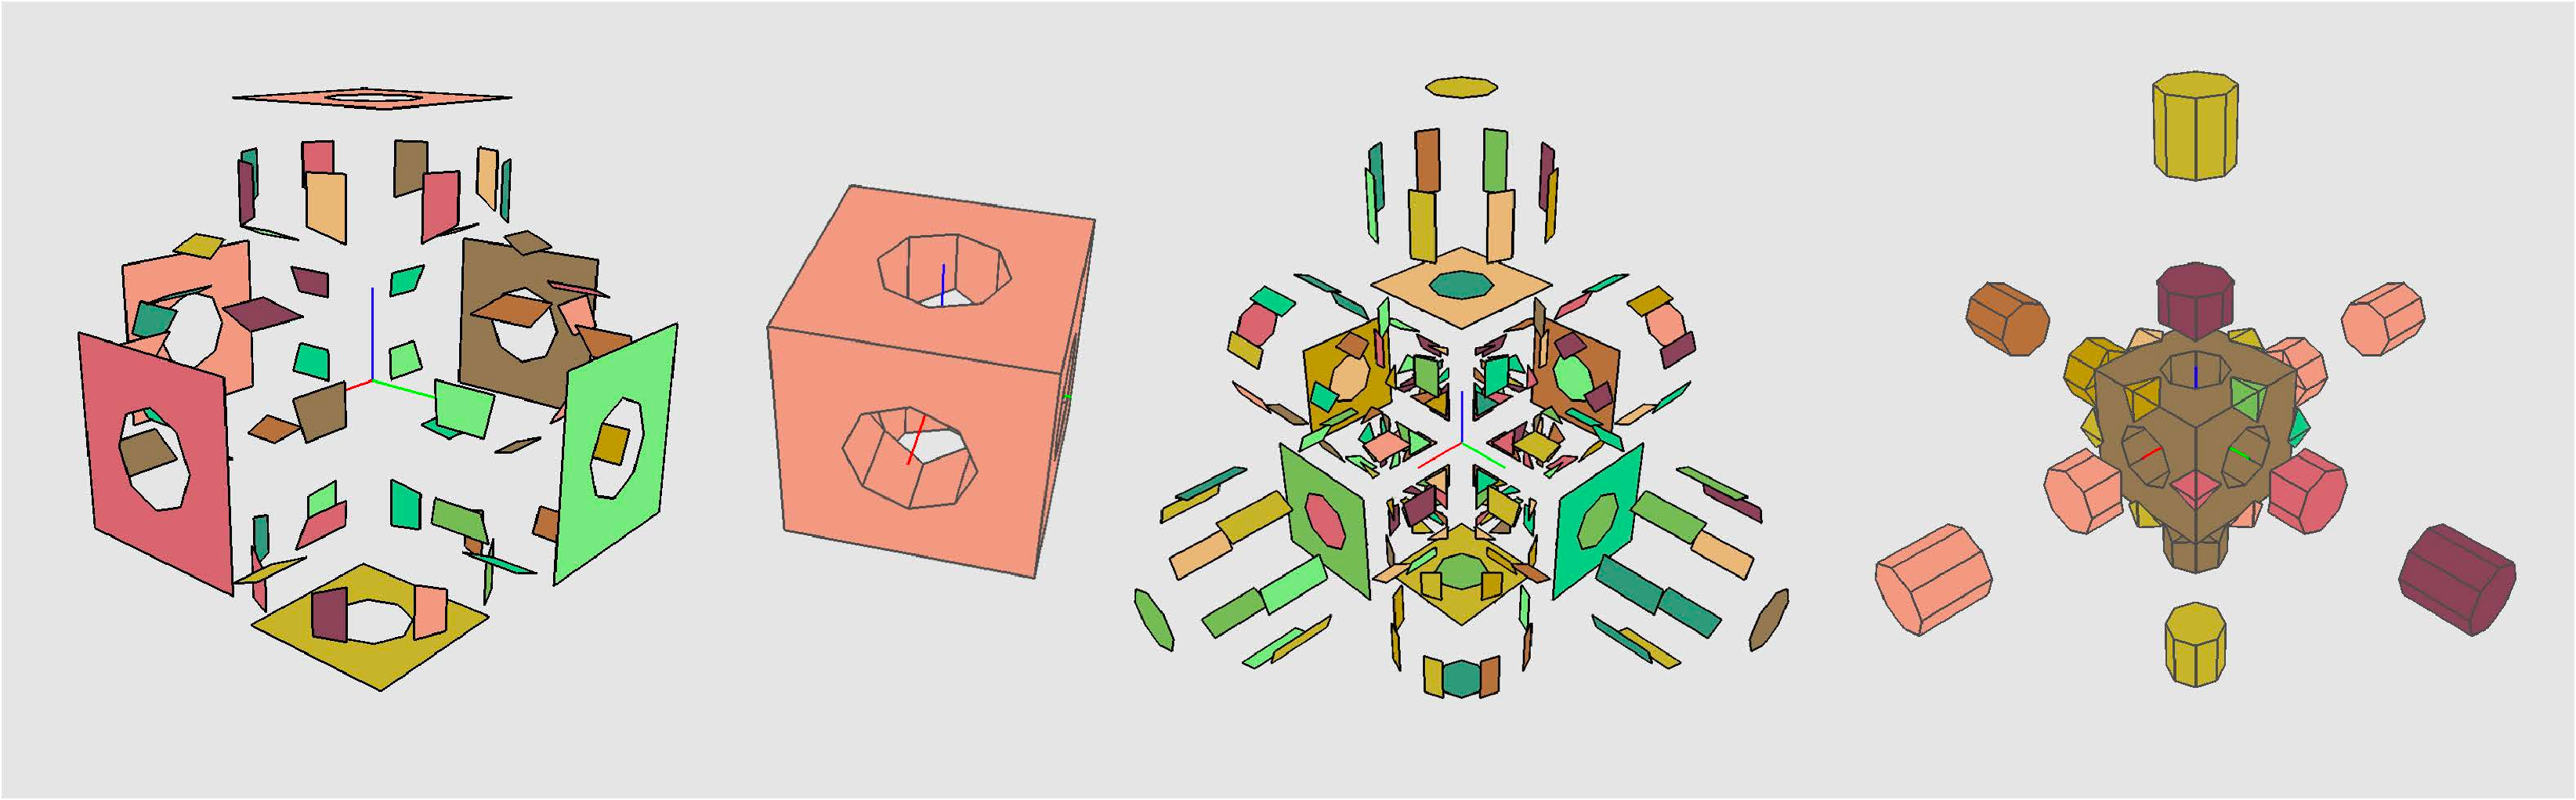
\includegraphics[width=0.95\linewidth]{figs/difference}%
		\caption{(a) {\tt result} of {\tt DIFFERENCE} exploded; (b) atom of {\tt DIFFERENCE result} exploded (just one); (c) {\tt UNION} exploded; (d) atoms of {\tt UNION result} exploded.}
		\label{fig:mech-2-diff}
	\end{figure*}

	\begin{figure}[h]
		\centering
		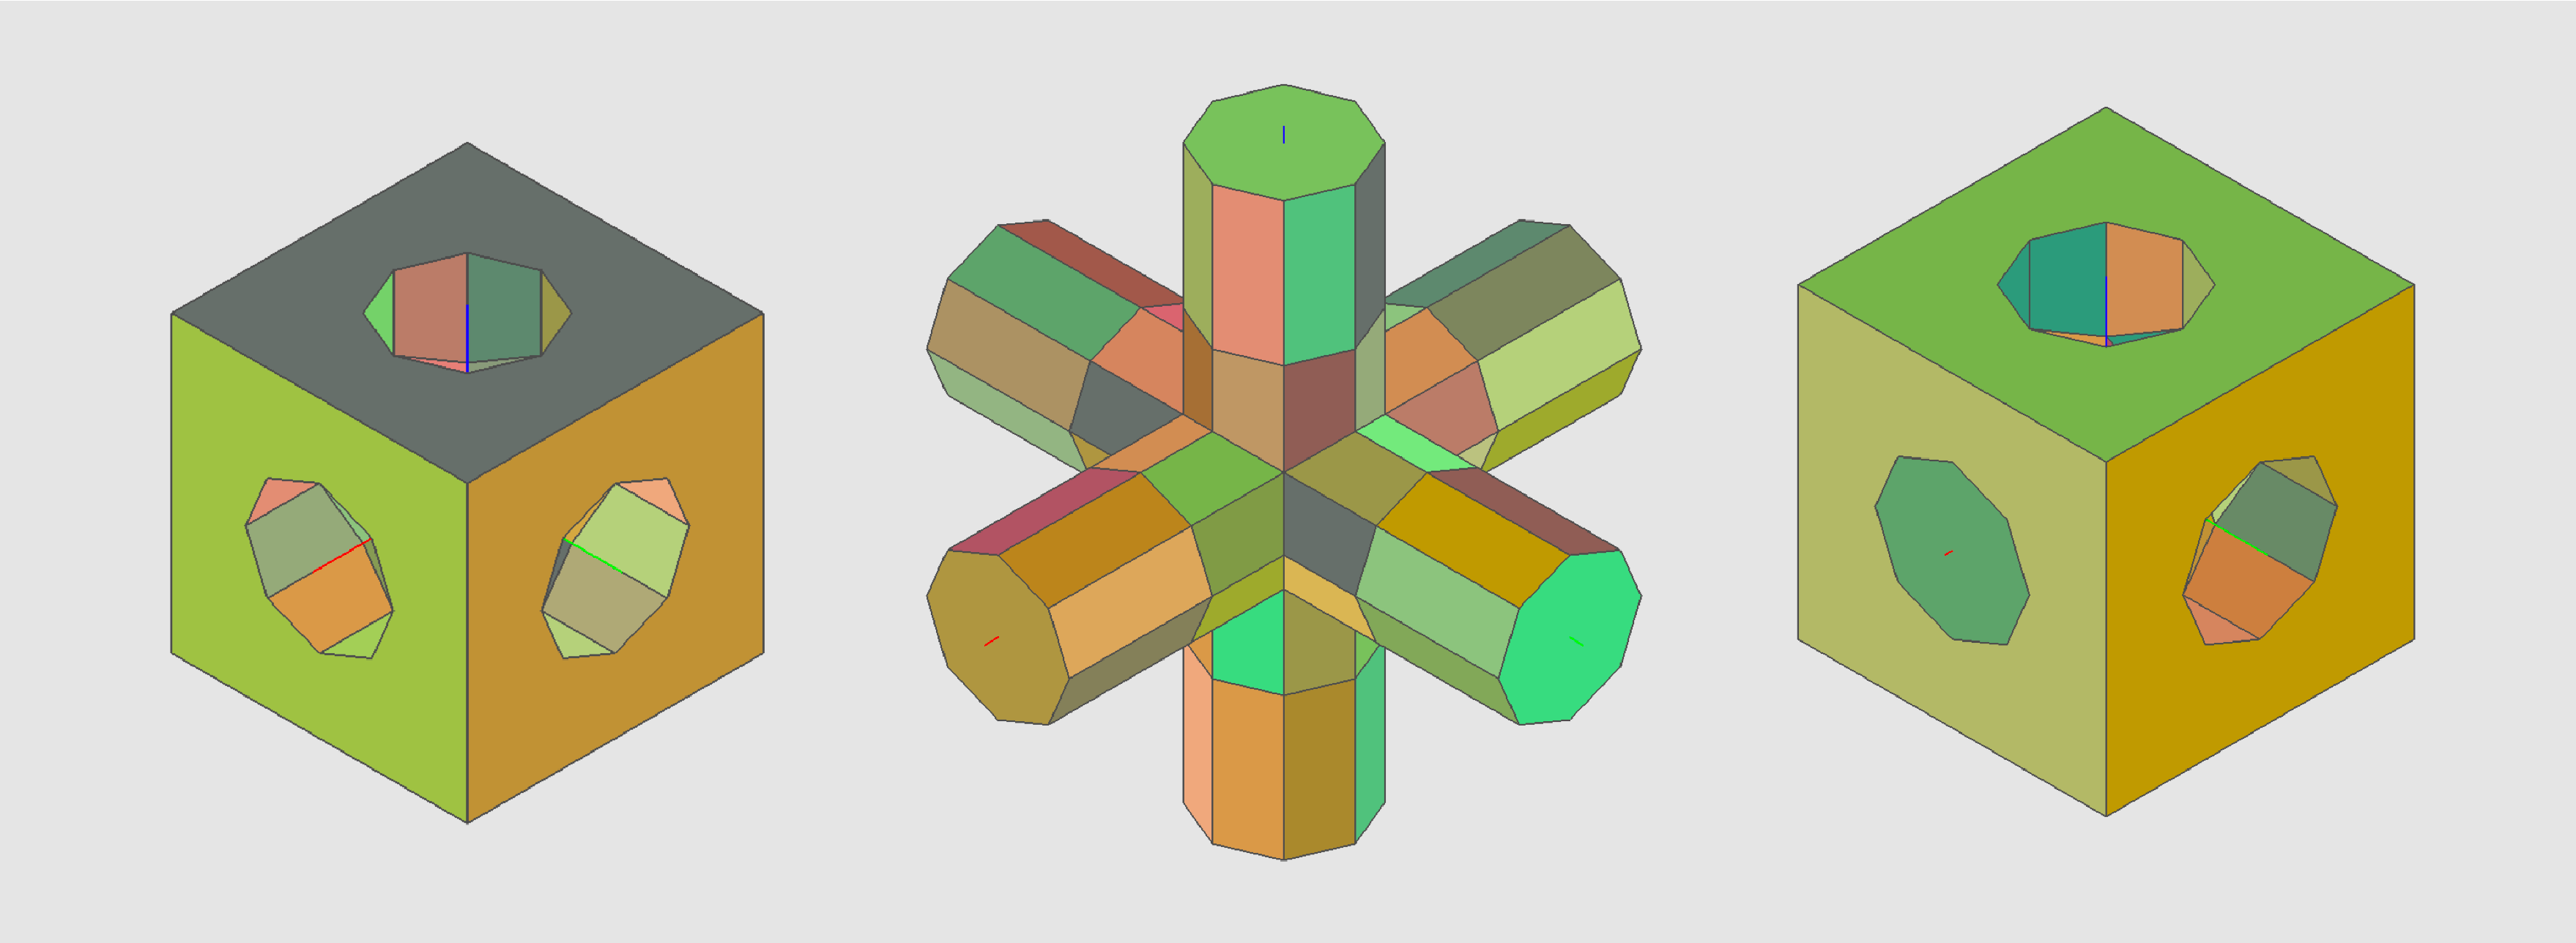
\includegraphics[width=0.95\linewidth]{figs/threecubes}%
		\caption{(a) {\tt c$\backslash$(x1$\cup$x2$\cup$x3)}; (b) {\tt x1$\cup$x2$\cup$x3}; (c) {\tt c$\backslash$(x2$\cup$x3)}, where {\tt c, x1, x2, x3} are the algebra generators.}
		\label{fig:mech-2-union}
	\end{figure}



\bibliographystyle{juliacon}
\bibliography{ref}

%% **************GENERATED FILE, DO NOT EDIT**************

\bibliographystyle{juliacon}
\bibliography{ref.bib}



\appendix

\section{Parametric building frame}
\label{sec:additional_doc}

Parametric models and topological operators demonstrate how to create flexible and reusable designs using parametric functions and topological transformations.
Geometric mapping of complexes and grids lets us explore techniques to map and manipulate geometric data structures effectively. Look at Figure \ref{fig:cad25}.

\begin{figure}[htbp]
	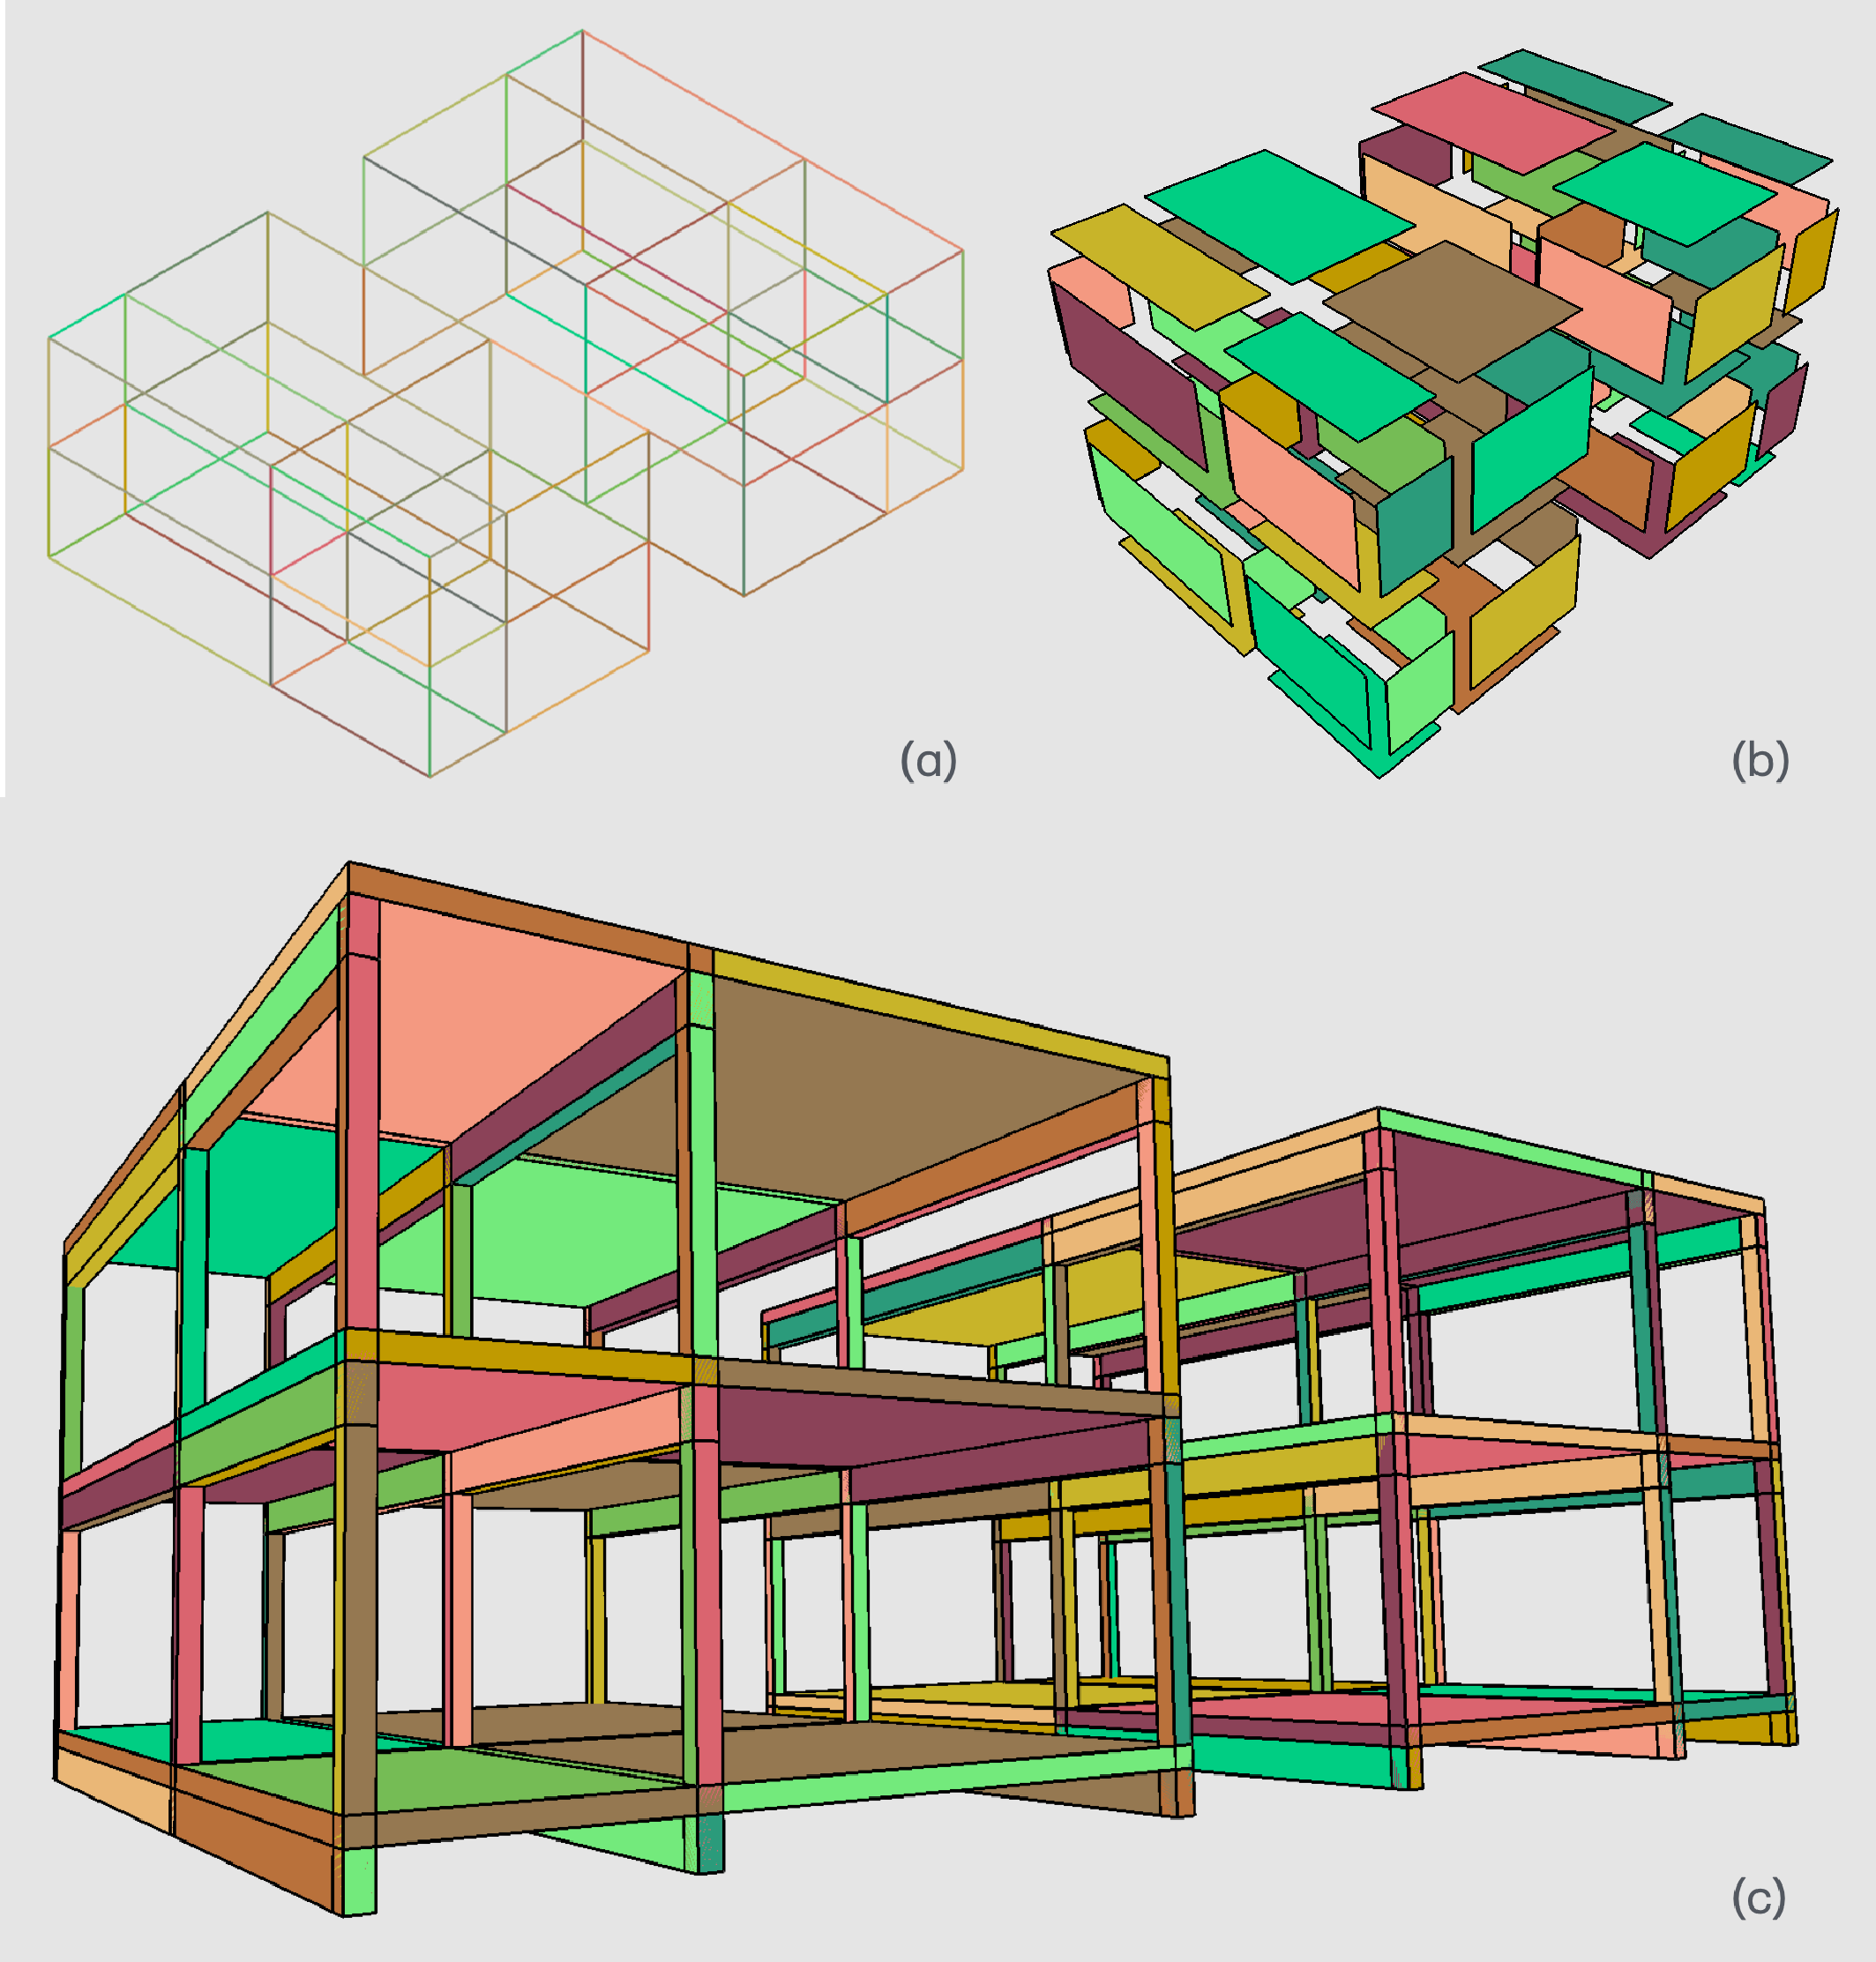
\includegraphics[width=\linewidth]{figs/cad25-building}
	\caption{(a) {\sf SK(1)(idea)}; (b) exploded object 2-complex; (c) structural {\sf framexyz} model from the project named {\sf idea} in the following Julia {\sf Plasm} fragment. All the generating {\sf Plasm} code is shown in Figure \ref{fig:plasmcode}.}
	\label{fig:cad25}
\end{figure}

\begin{figure}[t!]
\begin{center}
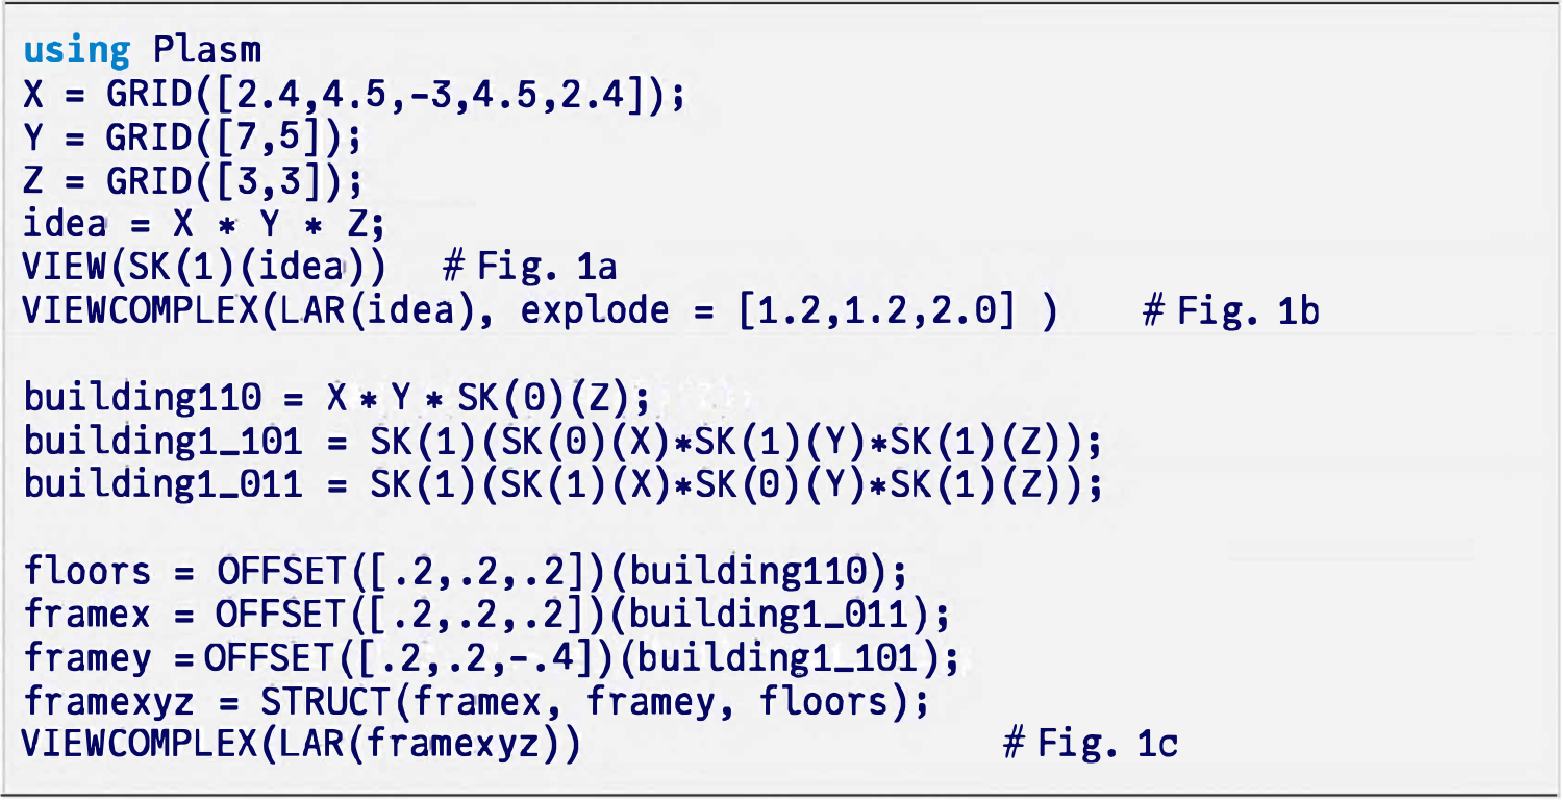
\includegraphics[width=\linewidth]{figs/building-2.pdf}
\caption{The Julia {\sf Plasm} code fragment producing all the images of Fig.~\ref{fig:images} .}
\end{center}
\label{fig:plasmcode}
\end{figure}

\vadjust{\vfill\pagebreak}


\end{document}

% Inspired by the International Journal of Computer Applications template
